% Cal Poly Thesis
% 
% based on UC Thesis format
%
% modified by Mark Barry 2/07.
%

\documentclass[12pt]{ucthesis}

\usepackage{amssymb}
\usepackage{amsmath}
\usepackage[letterpaper]{geometry}
\usepackage[overload]{textcase}
\usepackage{enumitem}
\usepackage{listings}
\usepackage{ifpdf}
\ifpdf
    \usepackage[pdftex]{graphicx}
    \graphicspath{ {./images/} }
    % Update title and author below...
    \usepackage[pdftex,plainpages=false,pdfpagelabels,breaklinks=true,colorlinks=true,urlcolor=blue,citecolor=blue,%
                                       linkcolor=blue,bookmarks=true,bookmarksopen=true,%
                                       bookmarksopenlevel=3,pdfstartview=FitV,
                                       pdfauthor={Alexander Paul Sideropoulos},
                                       pdftitle={dCAMP: Distributed Common API for Measuring Performance},
                                       pdfkeywords={thesis, masters, cal poly, distributed computing, performance monitoring}
                                       ]{hyperref}
    %Options with pdfstartview are FitV, FitB and FitH
    \pdfcompresslevel=1
\else
    \usepackage{graphicx}
\fi

% no line spacing with lists
\setlist{nolistsep}

\setlength{\parindent}{0.25in} \setlength{\parskip}{6pt}

\geometry{verbose,nohead,tmargin=1.25in,bmargin=1in,lmargin=1.5in,rmargin=1.3in}

\setcounter{tocdepth}{2}

% Different font in captions (single-spaced, bold) ------------
\newcommand{\captionfonts}{\small\bf\ssp}

\makeatletter  % Allow the use of @ in command names
\long\def\@makecaption#1#2{%
  \vskip\abovecaptionskip
  \sbox\@tempboxa{{\captionfonts #1: #2}}%
  \ifdim \wd\@tempboxa >\hsize
    {\captionfonts #1: #2\par}
  \else
    \hbox to\hsize{\hfil\box\@tempboxa\hfil}%
  \fi
  \vskip\belowcaptionskip}
\makeatother   % Cancel the effect of \makeatletter
% ---------------------------------------

%custom commands
\newcommand{\camp}{\emph{CAMP }}
\newcommand{\dcamp}{\emph{dCAMP }}

\begin{document}

% Declarations for Front Matter

% Update fields below!
\title{dCAMP: Distributed Common API for Measuring Performance}
\author{Alexander Paul Sideropoulos}
\degreemonth{June} \degreeyear{2014} \degree{Master of Science}
\defensemonth{June} \defenseyear{2014}
\numberofmembers{3} \chair{Dr. Michael Haungs} \othermemberA{Dr. Gene Fisher} \othermemberB{Dr. David Janzen} \field{Computer Science} \campus{San Luis Obispo}
\copyrightyears{seven}

\maketitle

\begin{frontmatter}

% Custom made for Cal Poly (by Mark Barry).
\copyrightpage

% Custom made for Cal Poly (by Andrew Tsui).
\committeemembershippage

\begin{abstract}

Although the nearing end of Moore's Law has been predicted numerous times in the past \cite{schaller1997}, it will eventually come to pass. In forethought of this, many modern computing systems to become increasingly complex, distributed, and parallel. As software is developed on and for these complex systems, a common API is necessary for gathering vital performance related metrics while remaining transparent to the user, both in terms of system impact and ease of use. Several distributed performance monitoring and testing systems have been proposed and implemented by both research and commercial institutions. However, most of these systems do not meet several fundamental criterion for a truly useful distributed performance monitoring system: 1) variable data delivery models, 2) security, 3) scalability, 4) transparency, 5) completeness, 6) validity, and 7) portability \cite{zanikolas2005}. This work presents the Distributed Common API for Measuring Performance, \dcamp, as a solution to meet each of these criterion.

\end{abstract}



\begin{acknowledgements}

   Thank you...

\end{acknowledgements}

\addcontentsline{toc}{chapter}{Contents}
\tableofcontents

\listoftables
\listoffigures

\end{frontmatter}

\pagestyle{plain}

\renewcommand{\baselinestretch}{1.66}

% ------------- Main chapters here --------------------

\chapter{Introduction}
\label{introduction}

As the Internet has become more pervasive in today's business economy, there has been a natural trend of distributing
large, complex systems across multiple components locally and throughout the world. These systems are not always
homogeneous with respect to hardware architecture or even operating system, and development of these system can prove to
be quite difficult even with the best tools available. In order to effectively build these systems, software engineers
must be able to test their system for performance defects as well as bottlenecks. Additionally, distributed systems must
respond to changes in availability and work load on its individual nodes.

Distributed performance testing frameworks supply software practitioners and system administrators with tools to
evaluate the performance of a system from both black box and white box perspectives by publishing interfaces for
instrumenting, collecting, analyzing, and visualizing performance data across the distributed system and distributed
applications. Distributed performance monitoring frameworks, often considered part of the testing framework, provide a
black box interface into monitoring a distributed system or application and usually includes mechanisms for triggering
actions based on performance events. For the purpose of this work, the term distributed performance framework is
introduced to collectively refer to both distributed performance testing and distributed performance monitoring
frameworks.

\section{Distributed Performance Framework Criterion}

In order for practitioners and researchers alike to effectively choose a distributed performance framework, it is
necessary to have a set criteria for evaluation. Presented here is an extended criterion of the general requirements
presented by \cite{zanikolas2005} for grid systems. Data Delivery Models and Security have been taken directly from
their work. Scalability has been modified to only consider good performance as its goal while Low Intrusiveness has been
turned into Transparency. Extensibility has been removed from the list, and Completeness and Validity have been added.
This work provides an alternate definition for Portability.

\subsubsection{Data Delivery Models}

Monitoring information includes fairly static (e.g., software and hardware configuration of a given node) and dynamic
events (e.g., current processor load, memory), which suggests the use of different measurement policies (e.g., periodic
or on demand). In addition, consumer patterns may vary from sparse interactions to long lived subscriptions for
receiving a constant stream of events. In this regard, the monitoring system must support both pull and push data
delivery models.
\cite{zanikolas2005}

\subsubsection{Security}

Certain scenarios may require a monitoring service to support security services such as access control, single or mutual
authentication of parties, and secure transport of monitoring information.
\cite{zanikolas2005}

\subsubsection{Scalability}

Monitoring systems have to cope efficiently with a growing number of resources, events and users. This scalability can
be achieved as a result of good performance which guarantees that a monitoring system will achieve the needed throughput
within an acceptable response time in a variety of load scenarios.
\cite{zanikolas2005}

\subsubsection{Transparency}

Transparency refers to the lack of impact a distributed performance framework makes on the system being monitored. As
\cite{zanikolas2005} states, it is ``typically measured as a function of host (processor, memory, I/O) and network load
(bandwidth) generated by the collection, processing and distribution of events.'' If a framework lacks transparency it
will fail to allow the underlying distributed system to perform well and will produce inaccurate performance
measurements, thereby reducing its Scalability and destroying its Validity.

\subsubsection{Completeness}

The Completeness of a distributed performance framework refers to the exhaustiveness to which it gathers performance
metrics. At a minimum, a framework must provide interfaces for measuring and aggregating performance data about a
system's processor, memory, disk, and network usage. Several distributed performance frameworks provide further detailed
performance metrics about the given distributed system being monitored, but this is usually at the cost of Portability.

\subsubsection{Validity}

A distributed performance framework is only as good as the data is produces; if the sensors or gathering techniques are
inaccurate, then the data is useless at best, misleading at worst. Validity of a framework is achieved when the authors
of a framework provide formal verification of its accuracy.

\subsubsection{Portability}

A framework's ability to run on a completely heterogeneous distributed system without special considerations by the
practitioner is what this work defines as Portability. More specifically, a portable framework has a unified API
regardless of the system architecture, does not restrict itself to applications written in specific programming
languages, and does not require practitioners to manually instrument their application code. This black box
characteristic is vital for a viable distributed performance framework's effectiveness as it allows practitioners to
focus on the performance data and not on a myriad of APIs for various architectures or languages.

\section{\dcamp}
\label{dcamp}

The Distributed Common API for Measuring Performance (\dcampns) is a distributed performance framework built on top of
Mark Gabel and Michael Haungs' 2007 research on \emph{CAMP: a common API for measuring performance} \cite{gabel2007}.
The fundamental functionality of \camp is providing an accurate and ``consistent method for retrieving system
performance data from multiple platforms.''

\dcamp takes advantage of this functionality and the authors' work done in validating \campns's accuracy and adds the
core feature sets listed below. As shown in the analysis work presented in Chapter \ref{analysis}, \dcamp adds these
features while still maintaining minimal impact on the systems, processes, and networks being monitored.

The key contributions of the Distributed Common API for Measuring Performance are:

\begin{itemize}
\item a stateful performance API,
\item distributed performance data aggregation,
\item performance filters and triggers, and
\item simplistic fault tolerance.
\end{itemize}

\subsection{Terminology}
Knowing the following terminology will make it easier to understand and discuss the \dcamp project, its main goals, its
usage, its components, and its inner workings. 

\begin{description}

\item[Distributed Performance Testing Framework (DPTF),]
\item[Distributed Performance Monitoring Framework (DPMF),]
\item[Distributed Performance Framework (DPF):]

An DPTF or DPMF (collectively termed DPF) is a framework which allows its users to evaluate the performance of a system
from both black box and white box perspectives by publishing interfaces for instrumenting, collecting, analyzing, and
visualizing performance data across the distributed system and distributed applications. Typically, the framework
provides a black box interface into monitoring a distributed system or application and includes mechanisms for
triggering actions based on performance events. The \dcamp project is designed to be a DPF. 

\item[Performance Metric,]
\item[Performance Counter:]
Performance metrics are any data about a given node relating to its throughput, capacity, utilization, or latency. In
\dcampns, these are grouped into four different sets of performance metrics---global, network, disk, and
per-process---and a fifth set of inquiry metrics. They are described fully in section \ref{dcamp_metrics}. 

\item[Metric Aggregation:]
Metric aggregation is the process of combining metrics from multiple nodes into a single metric. Performance metrics,
while useful at an individual system granularity, can be rather limited in value for a DPF where the goal is measurement
of the distributed system as a whole. Metric aggregation provides a coarser granularity for the performance metrics,
calculating a sum, average, percent, or any other mathematically relevant operation across multiple nodes in the system. 

\item[Metric Calculation:]
Metric calculation is the process of combining identical metrics from multiple timestamps into a single metric. Various
equations and inputs are used to do this calculation, chosen depending on the type of metric and desired representation;
these equations are listed in Table \ref{tab:metric_types}.

\item[Filter,]
\item[Throttle,]
\item[Threshold:]
Filtering (or throttling or thresholding) provides a mechanism for reducing the amount of data sent between nodes of the
system. Filtering allows a user to specify when or at what point to report metrics from one level to its parent. For
example, a filter might be set to only report average CPU utilization that is over seventy-five percent. 

\item[\dcamp Node,]
\item[\dcamp Process:]
A single, independently running instance of \dcamp in the distributed system is called a \dcamp node or process. More
than one node may exist on a single computer. A node consists of the Node role and zero or more other \dcamp roles. 

\item[\dcamp Service:]
Services are a way of logically grouping functions within the \dcamp system, from performance metric sampling to \dcamp
system management. A description of all the \dcamp services can be found in section \ref{roles_and_services}. Each
service is implemented in \dcamp as an independent thread.

\item[\dcamp Role:]
Roles in the \dcamp system are groupings of one or more \dcamp services. There does not exist a one-to-one
relationship between roles and services; the \dcamp role-to-service mapping can be seen in Table
\ref{tab:role_to_services}.

\item[\dcamp Hierarchy:]
The \dcamp system is organized in a hierarchical pattern with respect to data movement and system control functionality.
The hierarchy can be thought of as a tree structure, with leaf nodes being at the top of the hierarchy and a single root
node at the bottom. Metric data moves down the hierarchy from leaves to the root; configuration data and control
commands move up from the root to the leaves. 

\item[\dcamp Level:]
Levels are a way of organizing the \dcamp hierarchy horizontally. Levels are defined by their distance from the root
node. For example, level one is one node away from the root node, or said another way, the first level is directly
``connected'' to the root node. The second level is two nodes away from the root node, or any node in the second level is
connected to the root node by another node (in the first level). This necessarily means the root is in level zero (all
by itself).

\item[Parent Node:]
Nodes are called parent nodes if there exists at least one node connected to it from a level of higher ordinal value.
For example, a node in level one with at least one node connected to it from level two is considered a parent node. The
root node is inherently a parent node. 

\item[Child Node:]
A node is called a child node if it is connected to another node in a level of lower ordinal value. For example, a node
in level one is connected to the root node (in level zero), so it is called a child node. The root node is the only
node in the \dcamp system which is not a child node. 

\item[\dcamp Configuration:]
The \dcamp configuration specifies everything about the system, including hierarchy levels, metrics, sampling periods,
reporting periods, filtering, communication details, etc. The configuration is set at the root node and then
distributed to the rest of the \dcamp system. Configuration details can be found in section \ref{configuration}. 

\item[ZeroMQ,]
\item[zmq,]
\item[\O MQ:]
ZeroMQ is a message queuing framework which allows a developer to build distributed systems by focusing on the data
and implementing simple design patterns.

\item[ZeroMQ Address:]
A \O MQ address is the combination of network host identifier (i.e. an IP Address or resolvable name) and Internet
socket port number. 

\item[ZeroMQ Endpoint:]
An endpoint is the combination of any ZeroMQ transport (\texttt{pgm}, \texttt{inproc}, \texttt{ipc}, or \texttt{tcp})
and a \O MQ address.

\item[Metric Collection,]
\item[Metric Sampling:]
Metric collection or sampling is the process of measuring metrics on a given node. 

\item[Metric Reporting:]
Metric reporting is the process of sending sampled metrics to a parent node.

\end{description}


\chapter{dCAMP}
\label{dcamp}

The Distributed Common API for Measuring Performance (\dcamp) is a distributed performance framework built on top of Mark Gabel and Michael Haungs' 2007 research on \emph{CAMP: a common API for measuring performance} \cite{gabel2007}. The fundamental functionality of \camp is providing an accurate and ``consistent method for retrieving system performance data from multiple platforms.'' \dcamp\ takes advantage of this functionality and the authors' work done in validating \camp's accuracy and adds the following core feature sets:
\begin{itemize}
\item Stateful Performance API
\item Distributed Performance Data Aggregation
\item Performance Filters and Triggers
\item Simplistic Fault Tolerance
\end{itemize}

\section{Terminology}
Knowing the following terminology will make it easier to understand and discuss the dCAMP project, its main goals, its usage, its components, and how it works. 

~\\ \textbf{Distributed Performance Testing Framework (DPTF), Distributed Performance Monitoring Framework (DPMF), Distributed Performance Framework (DPF):} An DPTF or DPMF (collectively termed DPF) is a framework which allows its users to evaluate the performance of a system from both black box and white box perspectives by publishing interfaces for instrumenting, collecting, analyzing, and visualizing performance data across the distributed system and distributed applications. Typically, the framework provides a black box interface into monitoring a distributed system or application and includes mechanisms for triggering actions based on performance events. The dCAMP project is designed to be an DPF. 

~\\ \textbf{Performance Metric:} Performance metrics are any data about a given node relating to its throughput, capacity, utilization, or latency. In dCAMP, these are grouped into four different sets of performance metrics (global, network, disk, and per-process) and a fifth set of inquiry metrics. They are described fully below. 

~\\ \textbf{Metric Collection, Metric Aggregation, Metric Calculation:} Metric collection (or aggregation or calculation) is the process of combining metrics from multiple nodes into a single metric. Performance metrics, while useful at an individual system granularity, can be rather limited in value for a DPF where the goal is measurement of the distributed system as a whole. Metric collection provides a coarser granularity for the performance metrics. Collection could calculate a sum, average, percent, or any other mathematically relevant operation across multiple nodes in the system. 

~\\ \textbf{Filter, Throttle, Threshold:} Filtering (or throttling or thresholding) provides a mechanism for reducing the amount of data sent between nodes of the system. Filtering allows a user to specify when or at what point to report metrics from one level to its parent. For example, a filter might be set to only report average CPU utilization that is over seventy-five percent. 

~\\ \textbf{dCAMP Node, dCAMP Process:} A single, independently running instance of dCAMP in the distributed system is called a dCAMP node or process. More than one node may exist on a single computer. A node consists of the Node role and zero or more other dCAMP roles. 

~\\ \textbf{dCAMP Role:} Roles are a way of logically grouping functions within the dCAMP system, from performance metric gathering to dCAMP system management. A description of all the dCAMP roles can be found below. 

~\\ \textbf{dCAMP Service:} Services in the dCAMP system are implementations of one or more dCAMP roles. There does NOT exist a one-to-one relationship between services and roles; the dCAMP service-to-role mapping can be seen below. Each services is implemented in dCAMP as a single Python class. 

~\\ \textbf{dCAMP Hierarchy:} The dCAMP system is organized in a hierarchical pattern with respect to data movement and system control functionality. The hierarchy can be thought of as a tree structure, with leaf nodes being at the top of the hierarchy and a single root node at the bottom. Metric data moves down the hierarchy from leaves to the root; configuration data and control commands move up from the root to the leaves. 

~\\ \textbf{dCAMP Level:} Levels are a way of organizing the dCAMP hierarchy horizontally. Levels are defined by their distance from the root node. For example, level one is one node away from the root node, or said another way, the first level is directly "connected" to the root node. The second level is two nodes away from the root node, or any node in the second level is connected to the root node by another node (in the first level). This necessarily means the root is in level zero (all by itself). 

~\\ \textbf{Parent Node:} Nodes are called parent nodes if there is at least one node connected to it from a level of higher ordinal value. For example, a node in level one with at least one node connected to it from level two is considered a parent node. The root node is inherently a parent node. 

~\\ \textbf{Child Node:} A node is called a child node if it is connected to another node in a level of lower ordinal value. For example, a node in level one is connected to the root node (in level zero), so it is called a child node. The root node is the only node in the dCAMP system which is NOT a child node. 

~\\ \textbf{Configuration:} The dCAMP configuration specifies everything about the system, including root node, hierarchy levels, metrics, sampling frequency, reporting frequency, filtering, communication details, etc. The configuration is set at the root node and then distributed to the rest of the dCAMP system. Configuration details can be found below. 

~\\ \textbf{Metric Sampling:} Metric sampling is the process of measuring metrics on a given node. 

~\\ \textbf{Metric Reporting:} Metric reporting is the process of sending sampled metrics to a parent node.

\section{\dcamp Metrics}
\subsection{Global Metrics}
Global metrics measure overall CPU, process, thread, and memory usage of the system.
\begin{itemize}
\item Node CPU usage 
\item Node free physical memory (KB) 
\item Aggregate average CPU usage (\dcamp) 
\item Aggregate free physical memory (percentage) (\dcamp)
\end{itemize}

\subsection{Network I/O Metrics}
Network metrics measure utilization of a given network interface on the system.
\begin{itemize}
\item Total bytes sent on the given interface 
\item Total packets sent on the given interface 
\item Total bytes received on the given interface 
\item Total packets received on the given interface 
\item Aggregate bytes sent (\dcamp) 
\item Aggregate packets sent (\dcamp) 
\item Aggregate bytes received (\dcamp) 
\item Aggregate packets received (\dcamp)
\end{itemize}

\subsection{Disk I/O Metrics}
Disk I/O metrics measure throughput of a given disk or partition on the system.
\begin{itemize}
\item Number of read operations on the given disk 
\item Number of write operations on the given disk 
\item Number of read operations on the given partition 
\item Number of write operations on the given partition 
\item Aggregate number of read operations (\dcamp) 
\item Aggregate number of write operations (\dcamp)
\end{itemize}

\subsection{Per-process Metrics}
Per-process metrics measure CPU, memory, and thread usage for a single process on the system.
\begin{itemize}
\item Number of major and minor page faults 
\item Process CPU utilization 
\item Process user mode CPU utilization 
\item Process privileged mode CPU utilization 
\item Size of the process' working set in KB 
\item Size of the used virtual address space in KB 
\item Number of threads contained in the process
\end{itemize}

\subsection{Inquiry Metrics}
Inquiry metrics provide a mechanism for enumerating various properties of the system.
\begin{itemize}
\item Enumeration of the available disk partitions 
\item Enumeration of the available physical disks 
\item Enumeration of the valid inputs to the network functions 
\item Number of CPUs in the system 
\item "process identifier" for the given pid 
\item "process identifier" for each running process launched from an executable of the given name
\end{itemize}


\chapter{Design}
\label{design}

\dcamp is designed to be simple and only add complexity where needed. This allows for quick and easy, large scale
testing, for example. Additionally, in order to be transparent, minimizing network traffic was an important concern.

To this end, \dcamp configuration and management protocols are designed to be human-readable and verbose; this makes
them easy to debug and modify as needed. The data protocol, while also human-readable in its current form, is terse with
respect to the number of required messages and can be easily modified to use a more compact encoding scheme.

\section{Architecture}

\dcamp is designed as a semi-centralized, hierarchical peer-to-peer system utilizing the pipe-flow architecture
pattern \cite{needed} in which leaf (\textit{Metric}) nodes of the hierarchy collect data, filter out extraneous data,
and send it up the pipe to a \textit{Collector} node which subsequently filters out more data and sends it up to another
\textit{Collector} or \textit{Root} node. This architecture is efficient in that unwanted data is discarded earlier in
the data path, reducing transport and processing costs.

\section{Requirements}

As with any software engineering project, it is vital to have clearly stated requirements. \dcamp is no different. Below
are the list of functional and non-functional requirements which guide its design and implementation.

\subsection{Functional}

\begin{enumerate}

\item Configuration and Management
      \begin{itemize}
      \item An interface to instantiate and administer the system MUST be provided.
      \item Topology coordination MUST be handled automatically.
      \item An interface for configuring metric collections MUST be provided.
      \end{itemize}

\item Metric Collection
      \begin{itemize}
      \item An API for stateful, aggregate metrics on top of CAMP must be provided.
      \item Filters and thresholds SHOULD be configurable at any level in the collection topology.
      \item Aggregation of metrics across nodes MUST be supported.
      \item Performance data SHOULD be written to log files on each node.
      \end{itemize}

\item Fault Tolerance
      \begin{itemize}
      \item The topology MUST sustain brief network disconnectivity of any node.
      \item The topology MUST handle entrance/exit of any node(s) in the system.
            \begin{itemize}
            \item \textit{Metric} nodes MUST be allowed to enter/exit topology at any time.
            \end{itemize}
      \item \textit{Root}/\textit{Collector} nodes (i.e. parents) MUST failover in case of extended disconnectivity.
            \begin{itemize}
            \item Loss of previously collected data SHOULD be minimized during failover.
            \end{itemize}
      \item Management node MAY be allowed to enter/exit topology at any time.
      \end{itemize}

\end{enumerate}

\subsection{Non-Functional}

\begin{itemize}

\item \textbf{Transparency:} \dcamp SHOULD introduce negligible performance impact on \textit{Metric} nodes.
\item \textbf{Accuracy:} \dcamp MUST accurately report performance of \textit{Metric} nodes (individual and aggregated).
\item \textbf{Scalability:} \dcamp SHOULD maintain its transparency and accuracy as it scales (i.e. the number of
      \textit{Metric} nodes increases).

\end{itemize}

\section{\dcamp Roles and Services}
\label{roles_and_services}

The \dcamp distributed system is comprised of one or more nodes, each executing a role. The role is essentially a named
grouping of a specific, known set of functionality or service. Roles have little to no actual run-time logic but simply
act as containers for the services; services manage ZeroMQ sockets, communicating with other services/nodes, and do the
real work of \dcamp.

\subsection{Services}

Each \dcamp service has a specific purpose, but its scope can vary depending on the node's level in the \dcamp topology.

For example, the Configuration service has a specific purpose of replicating the \dcamp configuration from the
\textit{Root} to every node in the system via three distinct scopes: root, branch, and leaf. As part of the
\textit{Root} node, the Configuration service acts as a master copy of the configuration and publishes new values as
needed. As part of a \textit{Collector} node, the Configuration service stores every update from the \textit{Root} (for
possible use if the \textit{Root} dies) but no other changes are allowed to be written. Lastly as part of a
\textit{Metric} node, only configuration updates relevant to the node are stored by the Configuration service.

\begin{itemize}

\item \textbf{Node}---rudimentary \dcamp functionality; handles topology communication, heartbeat monitoring, and failure
      recovery.
\item \textbf{Sensor}---local performance metric gathering; essentially the \dcamp layer on top of the OS and hardware
      performance APIs (accessed via CAMP).
\item \textbf{Filter}---performance metric filtering; provides throttling and thresholding of metrics.
\item \textbf{Aggregation}--—performance metric aggregation; provides collection of and calculation on metrics from
      multiple Sensor and/or Aggregation services.
\item \textbf{Management}--—primary entry-point for end-user control of \dcamp distributed system; this is the \dcamp
      instrument panel, providing basic administration functions (e.g. start, stop, etc.).
\item \textbf{Configuration}--—complete or partial configuration replication; provides topology and configuration
      distribution.

\end{itemize}

\subsection{Roles}

The \textit{Base} role must be running on each node for it to be part of the \dcamp distributed system. In this
document, a ``\textit{Base} node'' is defined as a \dcamp node which has not yet been configured, i.e. it has not joined
a running \dcamp system. All other roles are launched from within the \textit{Base} role; see Section
\ref{threading_model} for more details.

The \textit{Metric} role runs on the nodes from which performance metrics should be collected. The \textit{Collector}
role acts as an aggregation point in the system, combining performance data from multiple \textit{Metric} (and
\textit{Collector}) nodes and providing additional aggregated performance metrics.

There is only one \textit{Root} role active in the system; it acts as the master copy of the \dcamp configuration and
sole user-interface point. The \textit{Root} role is not strictly attached to any given node in the system. Rather, the
\textit{Root} role may dynamically move to any first-level \textit{Collector} node if the current \textit{Root} node
fails.

Depending on the use case and desired system performance, an administrator may choose to split roles across multiple
nodes or collapse them onto a single node. For example, a single node may act as \textit{Metric}, \textit{Collector},
and \textit{Root} for smaller systems while larger systems would employ dedicated \textit{Collector} nodes. The \dcamp
\hyperref[configuration]{Configuration} syntax easily provides this flexibility to the system administrator.

Table \ref{tab:role_to_services} lists the roles which can be executed by a \dcamp node and the services which they
implement.

\begin{table}
\begin{tabular}{l l}

\hline
\textbf{Role} & \textbf{Service(s)} \\
\hline

Root & Management, Aggregation, Filter, Configuration (Full) \\

Collector & Aggregation, Filter, Configuration (Full) \\

Metric & Sensor, Filter, Configuration (Partial) \\

Base & Node \\

\end{tabular}
\caption{Role to Service Mappings}
\label{tab:role_to_services}
\end{table}

\section{Fault Tolerance}

In order to maintain a healthy distributed topology, \dcamp quickly and efficiently recovers from node failures using
simple fault tolerance rules. These rules define how/when nodes are considered to have failed as well as the specific
steps for recovering and/or rebuilding the distributed topology.

\subsection{Heartbeating (Detecting Disconnections)}

\dcamp detects node failures or disconnections via a lack of messages, e.g. missed X consecutive messages or no messages
received after D seconds. All messages act as heartbeats, not just the special \texttt{HUGZ} messages. By designing the
protocols with this in mind, network traffic can be minimized.

The \dcamp node failure detection rules are the following:

\begin{itemize}
\item \textit{Metric} nodes MUST detect when their parent (\textit{Collector}) node disconnects.
      (\hyperref[algor_promo]{Promotion Algorithm})
\item The \textit{Root} node MAY detect when a \textit{Collector} node disconnects. (\hyperref[algor_promo]{Promotion
      Algorithm})
\item \textit{Collector} nodes MUST detect when the \textit{Root} node disconnects. (\hyperref[algor_elect]{Election
      Algorithm})
\item The \textit{Root} node MUST detect when a \textit{Metric} node rejoins the system.
      (\hyperref[algor_remind]{Reminder Algorithm})
\end{itemize}

Because of the nature of ZeroMQ sockets, \textit{Collector} nodes should not need to know when a child (\textit{Metric})
node disconnects---when the child node reenters the topology, it is simply reassigned underneath the \textit{Collector}
and resume its metric collection and reporting.

Alternative approaches to \textit{Collector} node failure detection are (A) use of an ephemeral time-to-live (TTL)
property stored by the Configuration service and (B) \textit{Collector}-to-\textit{Collector} heartbeating. (B)
introduces additional network traffic and cannot scale with sufficiently large topologies. Furthermore, the same
essential functionality is present in (A) as the TTL would propagate to all \textit{Collector} nodes via the
Configuration service.

While approach (A) provides an additional detection mechanism for Collector node disconnections (namely the
\textit{Root} would detect \textit{Collector} failures as the TTL expires), it is simpler and arguably no less resilient
to solely detect failures from the child node's perspective.

\subsection{Reminder Algorithm (\textit{Metric} Node Recovery)}
\label{algor_remind}

\textit{Metric} nodes can leave and enter the \dcamp system at any time. When they rejoin, they are placed back into the
same location within the topology so as to maintain as much consistency within the performance data as possible.

The crux of this algorithm is the group definitions within the \dcamp configuration: nodes are always defined to be
within a group, and the groups define the network topology. Essentially, this algorithm is incorporated into the
Topology protocol; no additional work is necessary.

\begin{enumerate}
\item \textit{Metric} node rejoins the system with \texttt{POLO} response to \textit{Root} node's \texttt{MARCO}
      message.
\item \textit{Root} node detects \textit{Metric} node is already part of \dcamp system.
\item \textit{Root} node (re)sends \texttt{ASSIGN} message to \textit{Metric} node.
\end{enumerate}

\textit{Collector} nodes will not be overloaded by this algorithm since \textit{Metric} nodes are statically defined in
groups via the \dcamp Configuration. As \textit{Metric} nodes disconnect and reconnect, the \textit{Collector} node
virtually always has the same child nodes beneath it.

\subsubsection{DETECTION}

Detecting when a \textit{Metric} node disconnects is not necessary. Rather the \textit{Root} node only needs to detect
when a \textit{Metric} node rejoins the \dcamp system, comparing the \textit{Metric} node's UUID to the UUID already
saved in the topology.

\subsection{Promotion Algorithm (\textit{Collector} Node Recovery)}
\label{algor_promo}

As with the Reminder Algorithm, this recovery relies heavily on the \hyperref[proto_topo]{Topology Management Protocol}.
When a \textit{Metric} node, M, detects its \textit{Collector} node, C, is down, 

\begin{enumerate}
\item M sends an \texttt{SOS} message to the \textit{Root} node, R.
\item If R has received an \texttt{SOS} message from more than 1/3 of C's group, the algorithm proceeds as per below.
\end{enumerate}

When the \textit{Root} node, R, detects one of the \textit{Collector} nodes has disconnected,

\begin{enumerate}
\item R broadcasts a \texttt{STOP} message to all nodes within C's group and clears the groups configuration from the
      \dcamp system.
\item R then broadcasts a \texttt{MARCO} message and begins rebuilding the group topology via the Topology protocol.
\end{enumerate}

\subsubsection{DETECTION}

M will use the \hyperref[proto_config]{Configuration Replication Protocol} (\texttt{HUGZ} message is sent when there are
no configuration updates) to detect when C disconnects. R will use the \hyperref[proto_data]{Data Flow Protocol}
(\texttt{DATA(type='HUGZ')} message is sent when no data is scheduled to be reported) to detect when any of its
\textit{Collector} nodes has disconnected. That is, if M or R receives no messages from C within D seconds, C is
considered disconnected.

\subsection{Election Algorithm (\textit{Root} Node Recovery)}
\label{algor_elect}

This recovery algorithm is based on the bully algorithm present by H. Garcia-Molina in \cite{bully}. Only
\textit{Collector} nodes participate in the election, initiated when a \textit{Collector} node, C, detects the
\textit{Root} node, R, is down.

\begin{enumerate}
\item C sends \texttt{WUTUP} message to all nodes whose UUID is higher than its own, expecting a \texttt{YO} message in
      response.
\item If C does not receive any \texttt{YO} messages,
      \begin{enumerate}
      \item C declares victory by sending \texttt{IWIN} message to all nodes, and
      \item C waits W seconds before transitioning to become the Root, allowing for another node to replace it as
            \textit{Root} via a separate election.
      \end{enumerate}
\item If C receives a \texttt{YO} message,
      \begin{enumerate}
      \item C waits for W seconds to receive an \texttt{IWIN} message from another node whose UUID is higher than its
            own.
      \item If no \texttt{IWIN} message is received, C resends its \texttt{WUTUP} message and goes through the election
            process again.
      \end{enumerate}
\end{enumerate}

Additionally,

\begin{itemize}
\item If C receives a \texttt{WUTUP} message from a node whose UUID is lower than its own, C responds with a \texttt{YO}
      message and then starts its own election.
\item If C receives an \texttt{IWIN} message from a node whose UUID is lower than its own, C immediately begins a new
      election.
\end{itemize}

\subsubsection{DETECTION}

C will use the \hyperref[proto_config]{Configuration Replication Protocol} (\texttt{HUGZ} message is sent when there are
no configuration updates) to detect when R disconnects. That is, if C receives no message from R within D seconds, R is
considered disconnected.

\section{\dcamp Metrics}
\label{dcamp_metrics}

The crux of any DPF are the performance metrics to which it provides access. This section lists the set of performance
metrics available via \dcamp. Metrics marked with ``(\emph{dCAMP})'' are extensions added by the \dcamp project to the
basic CAMP metrics. These provide a performance view of multiple nodes in the distributed network and are collected by
the Aggregation service rather than the Sensor service.

\subsubsection{Global Metrics}
Global metrics measure overall CPU, process, thread, and memory usage of the system.
\begin{itemize}
\item Node CPU usage
\item Node free physical memory
\item Aggregate average CPU usage (\dcamp)
\item Aggregate free physical memory (\dcamp)
\end{itemize}

\subsubsection{Network I/O Metrics}
Network metrics measure utilization of a given network interface on the system.
\begin{itemize}
\item Total bytes sent on the given interface
\item Total packets sent on the given interface
\item Total bytes received on the given interface
\item Total packets received on the given interface
\item Aggregate bytes sent (\dcamp)
\item Aggregate packets sent (\dcamp)
\item Aggregate bytes received (\dcamp)
\item Aggregate packets received (\dcamp)
\end{itemize}

\subsubsection{Disk I/O Metrics}
Disk I/O metrics measure throughput of a given disk or partition on the system.
\begin{itemize}
\item Number of read operations on the given disk
\item Number of write operations on the given disk
\item Number of read operations on the given partition
\item Number of write operations on the given partition
\item Aggregate number of read operations (\dcamp)
\item Aggregate number of write operations (\dcamp)
\end{itemize}

\subsubsection{Per-process Metrics}
Per-process metrics measure CPU, memory, and thread usage for a single process on the system.
\begin{itemize}
\item Number of major and minor page faults
\item Process CPU utilization
\item Process user mode CPU utilization
\item Process privileged mode CPU utilization
\item Size of the process' working set in KB
\item Size of the used virtual address space in KB
\item Number of threads contained in the process
\end{itemize}

\subsubsection{Inquiry Metrics}
Inquiry metrics provide a mechanism for enumerating various properties of the system.
\begin{itemize}
\item Enumeration of the available disk partitions
\item Enumeration of the available physical disks
\item Enumeration of the valid inputs to the network functions
\item Number of CPUs in the system
\item ``process identifier'' for the given PID
\item ``process identifier'' for each running process launched from an executable of the given name
\end{itemize}

\section{Configuration}
\label{configuration}

A main feature of \dcamp is the configuration language which gives a system administrator a concise, powerful tool for
defining its performance monitoring behaviour. Two primary sets of parameters are needed in this configuration: the set
of nodes to include in \dcamp and the set of metrics those nodes will collect.

While it would be possible for \dcamp to be designed such that branches of the distributed hierarchy are automatically
formed based on dynamic inputs (e.g. node locality, performance metric configuration, balance of network vs CPU/memory
impact), the approach taken in \dcamp gives the system administrator control over this parameter.

Specifically, nodes are defined in groups within the \dcamp configuration, and each group is defined to collect one or
more distinct performance metrics. This gives the system administrator the freedom to collect varying metrics from each
branch of the topology and/or collect metrics at varying sample periods.

\subsection{Node Specification}

Nodes may be specified individually (as ZeroMQ addresses) or as groups (IP subnets). Additionally, nodes may be included
or excluded based on host name or IP Address matching. Name matching does a case-insensitive comparison of the node's
host name; left, right, or whole name matching can be specified. Address matching checks that the node's IP Address
falls within a given subnet (i.e. IP Address and mask length).

\begin{figure}[H]
\vspace{+10pt}
\begin{verbatim}
  node-spec        = address / node-group
  address          = host ":" port
  host             = name / ip-address
  node-group       = name 1*( address / ( subnet ":" port ) ) *filter
  subnet           = ip-address "/" mask-length
  filter           = [ "+" / "-" ] ( name-match / subnet-match )
  name-match       = [ ( "L" / "R" / "W" ) SP ] name
  subnet-match     = subnet
\end{verbatim}
\vspace{-20pt}
\caption{Configuration File - Node Specification}
\label{fig:config_file_node}
\end{figure}

\subsection{Sample Specification}

Performance metric samples are specified as:

\begin{enumerate}
\item the node(s) on which to sample the data,
\item the rate at which data should be sampled,
\item the threshold past which data should be reported, and lastly
\item the actual performance metric to be sampled.
\end{enumerate}

The report threshold can be specified as ``hold and report every N seconds'' or ``report when the metric value is
greater/less than X''. When ``hold'' is specified (via an \texttt{*}), all metric values sampled during the time limit
are sent. Otherwise, the \texttt{<} or \texttt{>} character indicates the metric should only be reported when its
calculated value is less-than or greater-than the given threshold value.

\begin{figure}[ht]
\vspace{+10pt}
\begin{verbatim}
  sample-spec      = 1*sample
  sample           = sample-rate [ report-threshold ] metric
  sample-rate      = seconds
  report-threshold = ( "*" seconds ) / ( ( "<" / ">" ) 1*DIGIT )
  metric           = ( global-metric / process-metric process-name )
  global-metric    = "CPU" / "MEMORY" / "DISK" / "NETWORK"
  process-metric   = "PROC_CPU" / "PROC_MEM" / "PROC_IO"
  seconds          = 1*DIGIT "s"
\end{verbatim}
\vspace{-20pt}
\caption{Configuration File - Sample Specification}
\label{fig:config_file_sample}
\end{figure}

\subsubsection{Accumulative Time-Based Filtering Pitfall}

Filtering can be thought of being done in one of two ways: accumulatively or discretely. Accumulative means only one
final value is reported for each time range (e.g. collect every second but report every minute, so sixty samples are
combined into a single value and then sent). Discrete means each constituent value is sent for each time range, but they
are ``held'' until the time limit is reached.

However, accumulation is not valuable for monotonically increasing values--it is the same as just sampling at the slower
frequency. Accumulation is only valuable for non-monotonically increasing values, but in that case, one should find the
raw, monotonically increasing values from which it is calculated and collect that metric instead.


\chapter{Implementation}
\label{implementation}

\section{Requirements}

\subsection{Functional}

\begin{enumerate}

\item Configuration
      \begin{itemize}
      \item instantiation, administration
      \item topology coordination
      \item metric collection spec.
      \end{itemize}

\item Metric Collection
      \begin{itemize}
      \item \dcamp API on top of CAMP
      \item filters (at various levels), thresholds
      \item aggregation of metrics across nodes
      \item output to log file
      \end{itemize}

\item Fault Tolerance
      \begin{itemize}
      \item simple rules to handle failures
      \end{itemize}

\end{enumerate}

\subsection{Fault Tolerance}

\begin{enumerate}

\item Topology MUST sustain brief network disconnectivity of any node.
\item \textit{Metric} nodes MUST be allowed to enter/exit topology at any time.
\item \textit{Root}/\textit{Collector} nodes (i.e. parents) MUST failover in case of extended disconnectivity.
      \begin{itemize}
      \item Loss of previously collected data SHOULD be minimized during failover.
      \end{itemize}
\item Management node SHOULD be allowed to enter/exit topology at any time.

\end{enumerate}

\subsection{Testing}

\begin{itemize}

\item \textbf{Transparency:} \dcamp SHOULD introduce negligible performance impact on sensor nodes.
\item \textbf{Accuracy:} \dcamp MUST accurately report metrics/performance of sensor nodes (individual and aggregated).
\item \textbf{Scalability:} \dcamp SHOULD maintain its transparency and accuracy as it scales (i.e. the number of sensor
      nodes increases).
\item \textbf{Fault Tolerance:} \dcamp MUST successfully handle entrance/exit of any node(s) in the system.

\end{itemize}

\section{\dcamp Operation}

\subsection{Sequence of \dcamp Operation}
\label{operation_sequnce}

The following steps describe how the \dcamp system is turned on. The \textit{Base} nodes (other than the node assigned
to be the \textit{Root}) can be started at any time by using the \dcamp CLI, before or after the \textit{Root} node is
initialized. It is expected these \textit{Base} nodes are managed by a watchdog utility which automatically restarts the
node if it exits for any reason.

\begin{figure}[H]
\vspace{+10pt}
\begin{lstlisting}[language=bash,frame=single,basicstyle=\footnotesize\ttfamily]
#!/usr/bin/env bash
while [ true ]
do
    dcamp base --address localhost:56789
done
\end{lstlisting}
\vspace{-10pt}
\caption{Sample Watchdog Script}
\label{fig:sample_watchdog}
\end{figure}

\begin{enumerate}

\item User promotes a \textit{Root} node via the \dcamp CLI, specifying a configuration file and a \textit{Base} node's
      address.
\item \textit{Root} node connects to each \textit{Base} node and begins the ``discover'' \hyperref[proto_topo]{Topology
      Protocol}.
\item \textit{Base} nodes join the \dcamp system at any time, being assigned as \textit{Collector} or \textit{Metric}
      nodes in the topology.

\item \dcamp runs in a steady state, nodes entering or exiting the system at any time.

      \begin{itemize}
      \item Performance counters are sampled, filtered, reported, and logged by the Metric nodes at regular intervals
            according to the \hyperref[configuration]{\dcamp Configuration}.
      \item Performance counters received from child nodes are aggregated, filtered, reported, and logged by
            \textit{Collector} nodes at regular intervals according to the \dcamp Configuration.
      \item Performance counters received from child nodes are aggregated and logged by \textit{Root} node for later
	    processing (e.g. graphing metrics during a test scenario or correlating statistics with a distributed event
	    log).
      \end{itemize}

\item User stops \dcamp by using the \dcamp CLI command.
\item \textit{Root} node begins the ``stop'' Topology Protocol.
\item \textit{Collector} and \textit{Metric} nodes exit the topology and revert to \textit{Base} nodes.
\item \textit{Root} node exits, reverting to \textit{Base} node.

\end{enumerate}

\subsection{Threading Model}
\label{threading_model}

As mentioned above as the first and third steps of \dcamp operation, a \textit{Base} node can transform into one of the
three active \dcamp roles: \textit{Root}, \textit{Collector}, or \textit{Metric}. This transformation is actually the
\textit{Base} role (via the Node service) launching and managing another role internally. This interaction is depicted
in Figure \ref{fig:node_role_service_image}.

\begin{figure}[H]
    \centering
    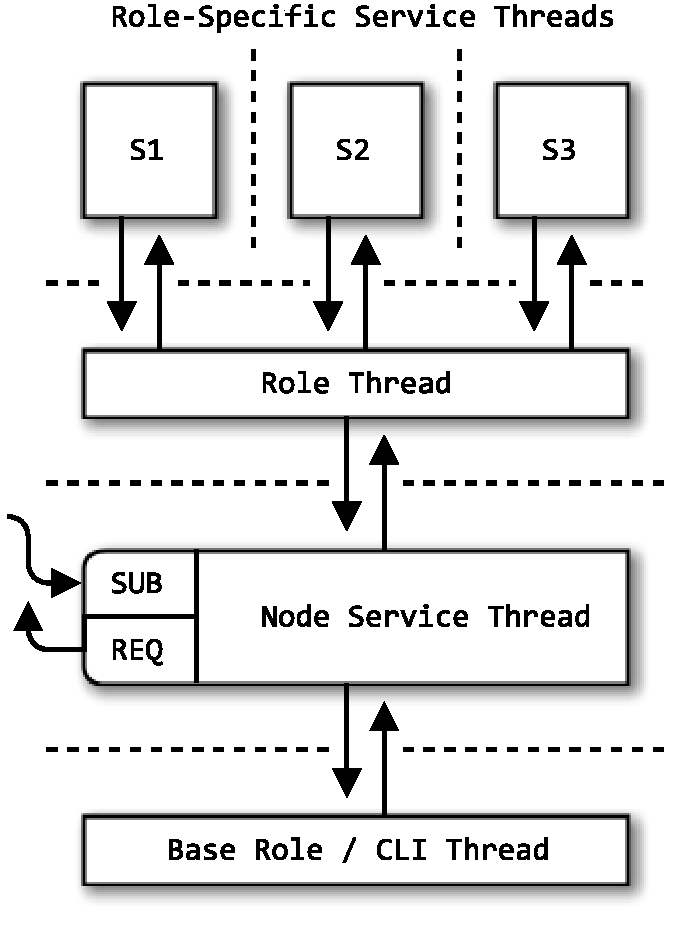
\includegraphics[scale=0.5]{node-role-service.pdf}
    \caption[Node, Role, Services Threading Model Diagram]
            {Node, Role, Services Threading Model Diagram: Thread boundaries are represented by dashed lines. Except for
	     the Node service's \texttt{SUB} and \texttt{REQ} sockets, all arrows represent \texttt{PAIR} socket
	     communication.}
    \label{fig:node_role_service_image}
\end{figure}

When a \textit{Base} node is running, only the bottom two threads (the \textit{Base} role and the Node service) are
active. Once it receives an assignment from the ``discover'' Topology Protocol or the \dcamp CLI, the Node service
launches an appropriate role thread which, in turn, launches one or more role-specific service threads.

All communication between the roles and services occurs across \texttt{PAIR} control sockets. There are also various
service-to-service communications which occur via \texttt{inproc} transport sockets (e.g. the internal
\hyperref[proto_data]{Data Flow Protocol}) and shared memory data structures (e.g. the Configuration service).

Also mentioned in section \ref{operation_sequnce} as the last two steps, each role exits and, by doing so, reverts
itself back to a \textit{Base} node. This is handled just like before, with the Node service receiving a \texttt{STOP}
message via the ``stop'' Topology Protocol and then notifying the internally running role to shut down. The role thread
then notifies its service threads, waits for them to finish, then exits.

\section{ZeroMQ Protocols}

For a quick background on ZeroMQ socket types and message patterns, please see Appendix \ref{zeromq_primer}.

\subsection{Topology Protocol}
\label{proto_topo}

The \dcamp distributed topology is dynamically established as the Root node sends out its discovery message and receives
join messages from Base nodes. Once a Base node responds to the Root, the Base node is given its assignment.
Additionally, the Root node can shutdown the system using this same protocol but responding with a "stop" message
instead of an assignment.

\begin{figure}[H]
\vspace{+10pt}
\begin{verbatim}
topo-discovery = *discover join
discover       = R-MARCO
join           = B-POLO ( R-ASSIGN / R-STOP / R-WTF )
\end{verbatim}
\vspace{-5pt}
\caption[Topology Protocol]
        {Topology Protocol: \texttt{R-} represents the Root node sending a message and \texttt{B-}
         represents a Base node sending a message.}
\label{fig:proto_topo_spec}
\end{figure}

\begin{figure}[H]
    \centering
    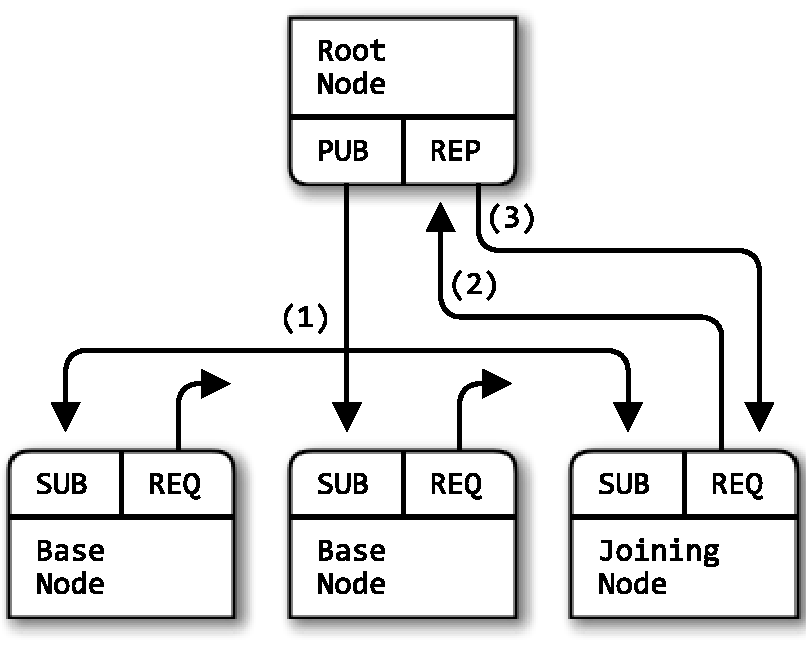
\includegraphics[scale=0.5]{topo.pdf}
    \label{fig:proto_topo_image}
    \caption{Topology Protocol Diagram}
\end{figure}

\subsubsection{Message Definitions}

\textbf{\texttt{TOPO}} is a generic topology message consisting of four frames. This message type is designed to be sent
across a PUB/SUB connection, from which subscribers filter incoming messages using the first frame. This design proves
useful for the \hyperref[proto_reco]{Recovery Protocols}.

The \texttt{MARCO} message is simply shorthand for \texttt{TOPO(key="/MARCO")}.

\begin{figure}[H]
\vspace{+10pt}
\begin{verbatim}
Frame 0: key, as 0MQ string
Frame 1: root address, as 0MQ string
Frame 2: root UUID, 16 bytes in network order
Frame 3: <empty> or content, as 0MQ string
\end{verbatim}
\vspace{-20pt}
\caption{\texttt{TOPO} Message Definition}
\label{fig:message_topo}
\end{figure}

\textbf{\texttt{CONTROL}} is a generic control message consisting of four frames and designed to be sent across a
REQ/REP connection. The \texttt{POLO}, \texttt{ASSIGN}, and \texttt{STOP} messages are shorthand for
\texttt{CONTROL(command="POLO")}, \texttt{CONTROL(command="ASSIGN")}, and \texttt{CONTROL(command="STOP")} respectively.

In the case of \texttt{ASSIGN}, the third frame contains the specific topology instructions (level-one collector, leaf
node, etc.) being sent to the Base node.

\begin{figure}[H]
\vspace{+10pt}
\begin{verbatim}
Frame 0: command, as 0MQ string
Frame 1: base address, as 0MQ string
Frame 2: base UUID, 16 bytes in network order
Frame 3: properties, JSON-encoded, as 0MQ string

command     = "polo" / "assignment"
properties  = *( parent / level / group )
parent      = "parent=" <node-address>
level       = "level=" ( "root" / "branch" / "leaf" )
group       = "group=" <group-identity>
\end{verbatim}
\vspace{-20pt}
\caption{\texttt{CONTROL} Message Definition}
\label{fig:message_control}
\end{figure}

\textbf{\texttt{WTF}} is \dcamp's error message type. It has three frames (though Frame 2 may be empty) with the first
designed to make error detection simple.

\begin{figure}[H]
\vspace{+10pt}
\begin{verbatim}
Frame 0: "WTF", as 0MQ string
Frame 1: error code, 4 bytes in network order
Frame 2: <empty> or error message, as 0MQ string
\end{verbatim}
\vspace{-20pt}
\caption{\texttt{WTF} Message Definition}
\label{fig:message_wtf}
\end{figure}

\subsection{Configuration Replication Protocol}
\label{proto_config}

\dcamp configuration and topology state are replicated across the system using key-value pairs, with the keys laid out
in a hierarchical fashion. This lends itself nicely to PUB/SUB topic filtering.

For example, because a Metric node only needs the configuration values for its particular group, the node subscribes
only to the \texttt{"/CONFIG/<group-name>/"} topic. Any \texttt{KVPUB} whose key does not start with this string is
then discarded.

In practice, Metric nodes need more than just their group-specific configuration, but the general principle holds true:
nodes only receive the configuration data they require and nothing more. In the case of first-level Collector nodes, they
receive all updates since they are fail-over candidates for the root node.

\begin{figure}[H]
\vspace{+10pt}
\begin{verbatim}
config-replication = *update / snap-sync
update             = P-KVPUB / P-HUGZ
snap-sync          = C-ICANHAZ ( ( *P-KVSYNC P-KTHXBAI ) / P-WTF )
\end{verbatim}
\vspace{-5pt}
\caption[Configuration Protocol Specification]
	{Configuration Protocol Specification: \texttt{P-} represents the parent node (Root or Collector) sending a
	 message and \texttt{C-} represents the child node sending a message.}
\label{fig:proto_config_spec}
\end{figure}

A newly assigned first-level Collector node will first subscribe to new configuration updates from the Root node and
then send a configuration snapshot request to the Root node. A newly assigned Sensor (or non-first-level Collector) node
will first subscribe to new configuration updates from its parent Collector node, and then send its parent Collector
node a filtered configuration snapshot request. Once its snapshot has been successfully received, a node will process
any pending configuration updates and then, in the case of a Collector node, respond to child node snapshot requests.

The \dcamp configuration replication algorithm adheres to the Clustered Hashmap Protocol\cite{chp} with a few minor
(and one major) modifications:

\begin{enumerate}
\item only the Root node may write updates to the configuration,
\item the full configuration table will be replicated across all first-level Collector nodes (lower-level nodes may
      filter their configuration to only store relevant data),
\item a different set of command names are used (as described below), and
\item configuration updates are distributed via the \dcamp hierarchy (instead of directly from the Root node).
\end{enumerate}

\begin{figure}[H]
    \centering
    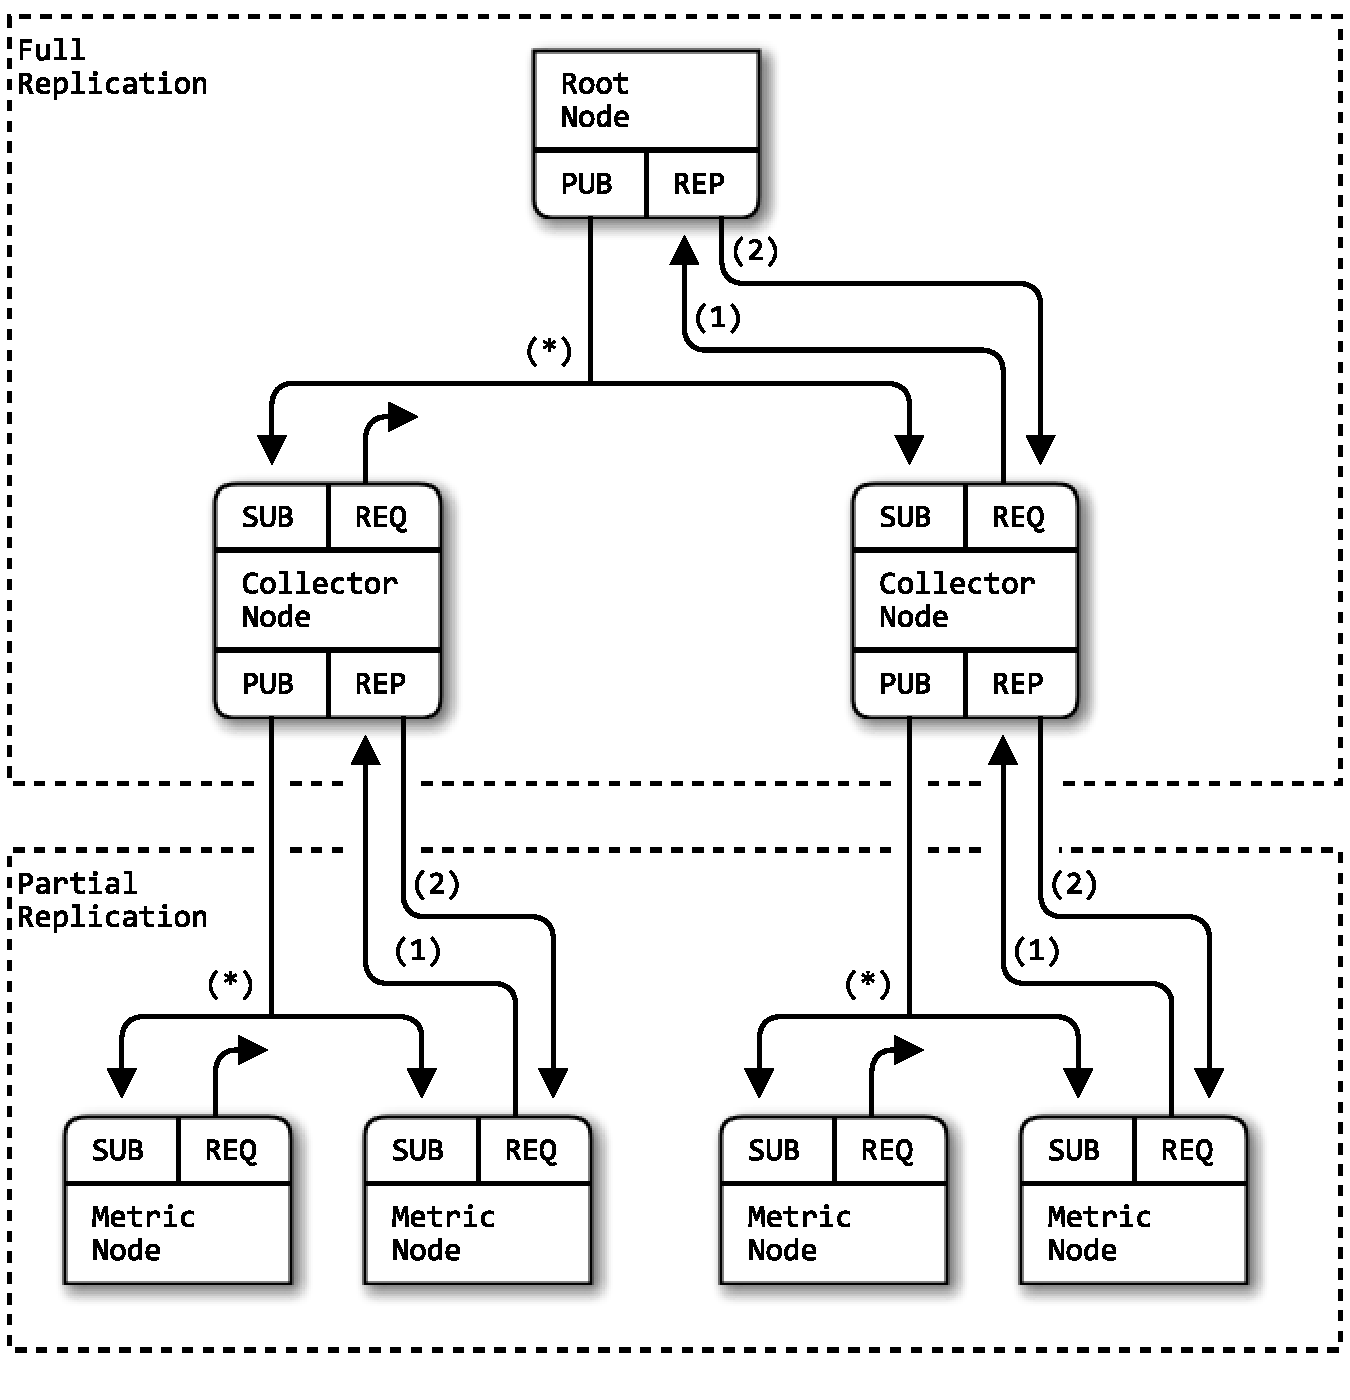
\includegraphics[scale=0.5]{config.pdf}
    \caption{Configuration Protocol Diagram}
    \label{fig:proto_config_image}
\end{figure}

\subsubsection{Message Definitions}

These messages come from the CHP protocol. Additionally, a \texttt{WTF} error message may be sent by the parent in case
of error. It should be noted, each of the following messages is really the same five-frame format with varying keys and
semantics.

As shown in Figure \ref{fig:proto_config_spec}, the \texttt{ICANHAZ}, \texttt{KVSYNC}, and \texttt{KTHXBAI} messages are
sent across a REQ/REP connection type. \texttt{KVPUB} (as the name would imply) along with the \texttt{HUGZ} heartbeat
message are designed for the PUB/SUB pattern.

\textbf{\texttt{ICANHAZ}} is a configuration snapshot request sent by the child node when it first starts. Multiple
\texttt{ICANHAZ} requests can be sent for the different topics or subtrees needed by the node, and the node will not
begin normal operation until all of the requested values have been received.

\begin{figure}[H]
\vspace{+10pt}
\begin{verbatim}
Frame 0: "ICANHAZ", as 0MQ string
Frame 1: <empty>
Frame 2: <empty>
Frame 3: <empty>
Frame 4: subtree specification, as 0MQ string
\end{verbatim}
\vspace{-20pt}
\caption{\texttt{ICANHAZ} Message Definition}
\label{fig:message_icanhaz}
\end{figure}

\textbf{\texttt{KVSYNC}} is a configuration snapshot response message. For every key-value pair within the requested
subtree, a \texttt{KVSYNC} message is sent to the child node. Note: if no values exist for a requested subtree, a
\texttt{KTHXBAI} message will be the only response received by the child node.

The sequence number in Frame 1 SHOULD be ignored by the recipient since no order guarantees exist for configuration
snapshots requests.

\begin{figure}[H]
\vspace{+10pt}
\begin{verbatim}
Frame 0: key, as 0MQ string
Frame 1: sequence number, 8 bytes in network order
Frame 2: <empty>
Frame 3: <empty>
Frame 4: value, as blob
\end{verbatim}
\vspace{-20pt}
\caption{\texttt{KVSYNC} Message Definition}
\label{fig:message_kvsync}
\end{figure}

\textbf{\texttt{KTHXBAI}} marks the end of a successful snapshot request. Frame 4 MUST contain the highest sequence
number of all the values in the configuration snapshot.

\begin{figure}[H]
\vspace{+10pt}
\begin{verbatim}
Frame 0: "KTHXBAI", as 0MQ string
Frame 1: sequence number, 8 bytes in network order
Frame 2: <empty>
Frame 3: <empty>
Frame 4: subtree specification, as 0MQ string
\end{verbatim}
\vspace{-20pt}
\caption{\texttt{KTHXBAI} Message Definition}
\label{fig:message_kthxbai}
\end{figure}

\textbf{\texttt{KVPUB}} is a configuration update sent from parent to child. The sequence number in Frame 1 must be
monotonically increasing. When a \texttt{KVPUB} is received which has a sequence number lower than a previously received
\texttt{KVPUB}, the node MUST delete its saved configuration values and request a new snapshot.

Frame 2 SHOULD contain the UUID of the node from which the value originated. In \dcamp, this should only be the Root
node's UUID. Frame 3 MAY contain additional properties for the key-value pair, such as an ephemeral time-to-live.

\begin{figure}[H]
\vspace{+10pt}
\begin{verbatim}
Frame 0: key, as 0MQ string
Frame 1: sequence number, 8 bytes in network order
Frame 2: UUID, 16 bytes in network order
Frame 3: properties, JSON-encoded, as 0MQ string
Frame 4: value, as blob
\end{verbatim}
\vspace{-20pt}
\caption{\texttt{KVPUB} Message Definition}
\label{fig:message_kvpub}
\end{figure}

\textbf{\texttt{HUGZ}} is the heartbeat message sent from parent to child when the rate of \texttt{KVPUB} messages being
sent drops below a predetermined threshold. The \texttt{HUGZ} message is critical to maintaining topological consistency
in \dcamp.

\begin{figure}[H]
\vspace{+10pt}
\begin{verbatim}
Frame 0: "HUGZ"
Frame 1: 00000000
Frame 2: <empty>
Frame 3: <empty>
Frame 4: <empty>
\end{verbatim}
\vspace{-20pt}
\caption{\texttt{HUGZ} Message Definition}
\label{fig:message_hugz}
\end{figure}

\subsection{Data Flow Protocol}
\label{proto_data}

There are two data flow protocols in the \dcamp system: the external protocol for data flowing from one node to the next
(via PUB/SUB) and the internal protocol for data flowing between components of a single node (via PUSH/PULL). Both
protocols have the same specification and use the same message formats.

\begin{figure}[H]
    \centering
    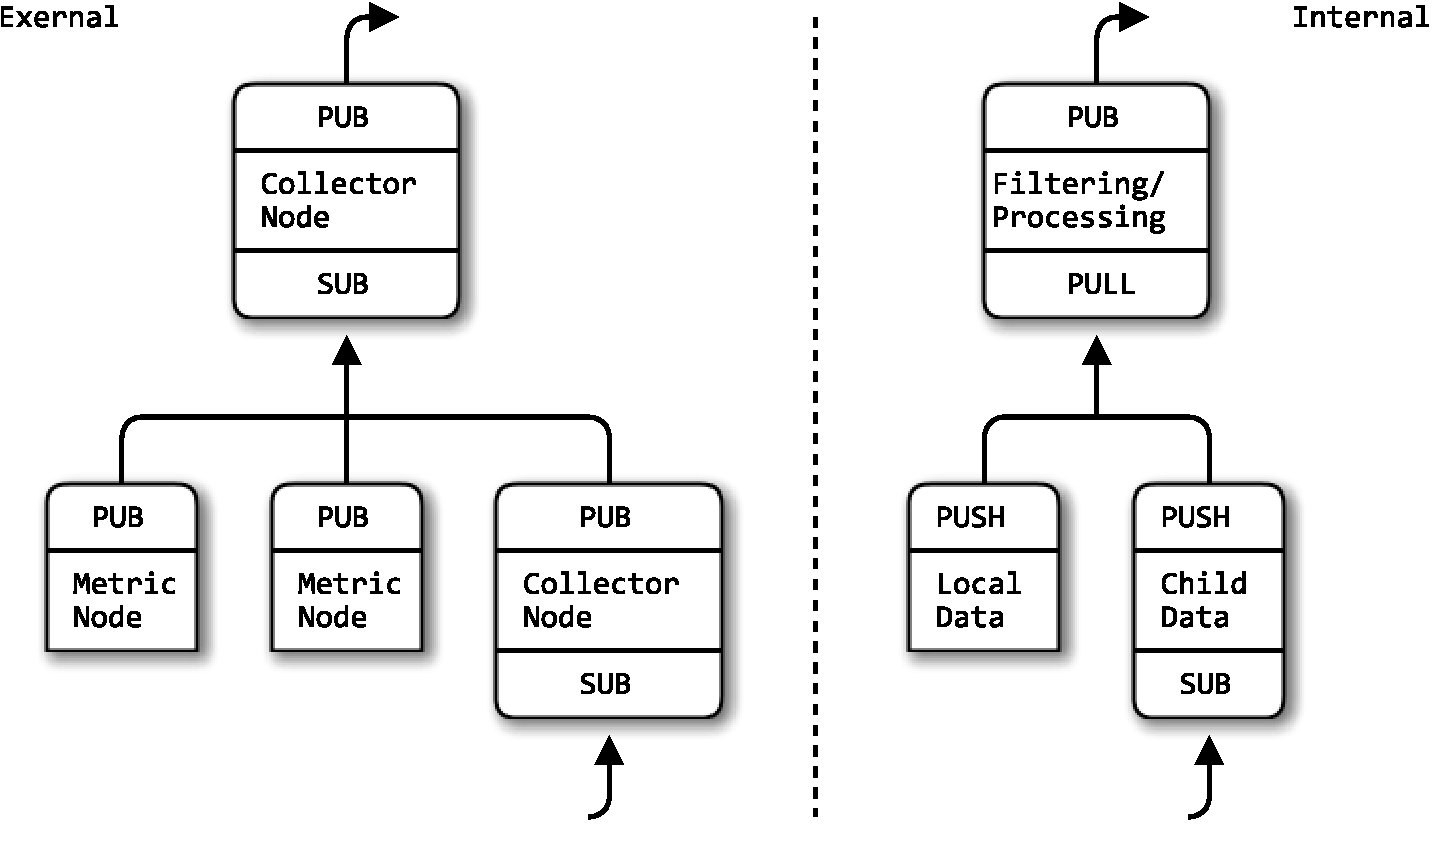
\includegraphics[scale=0.5]{data.pdf}
    \caption{Data Flow Diagram}
    \label{fig:proto_data_image}
\end{figure}

The \dcamp data flow protocol is very simple, comprised of a single data message type. The data flows from one node to
another via PUB/SUB sockets. Internally, data flows from the upstream data producers, through a filtering/processing
unit, and out to downstream data consumers via PUSH/PULL sockets.

When data rate is slower than a predefined threshold, heartbeats are sent instead to keep inter-node connections alive.

\begin{figure}[H]
\vspace{+10pt}
\begin{verbatim}
data-flow = *( METRIC / HUGZ )
\end{verbatim}
\vspace{-5pt}
\caption[Data Flow Specification]
	{Data Flow Specification: All messages are sent from child (Metric or Collector) to parent (Collector or Root).}
\label{fig:proto_data_spec}
\end{figure}

\subsubsection{Performance Measurement}

When discussing performance measurement, it is important to understand how metrics are sampled, calculated, and
presented to an end user.

Performance metrics, also called counters, are usually monotonically increasing values. That is, reading its raw,
instantaneous value is virtually meaningless; to correctly read the counter it must be sampled at two different points
in time and then calculated.

For example, when displaying a graph of data point for non-basic metric types, each data point is really a calculated
value of the value at the current timestamp and that at the previous timestamp. It is possible to look at fewer data
samples to first get a course-grain view (e.g. five-minute samples) of the metric before drilling in a looking at
finer-grain samples (e.g. one-second samples).

Non-monotonically increasing counters do exist (e.g. disk speed, Ethernet uplink speed, etc.), but these are usually
fairly static configuration values and do not need to be sampled frequently. \dcamp supports these types of counters
with the ``basic'' metric type.

Table \ref{tab:metric_types} shows how each of the \dcamp metric types are calculated. Note: unlike some other
performance measurement frameworks\cite{ganglia}, \dcamp stores all metrics in their raw, uncalculated form and only
presents a calculated value upon display.

\renewcommand{\arraystretch}{1.5}
\begin{table}
\begin{tabular}{ l|l|l }
\hline
\textbf{Type} & \textbf{Contents of Single Sample} & \textbf{Calculation of Two Samples}
\tabularnewline
\hline
basic & raw value at specified timestamp & \( C = V_{t_2} \)
\tabularnewline
delta & raw value at specified timestamp & \( C = V_{t_2} - V_{t_1} \)
\tabularnewline
rate & raw value at timestamp & \( C = \frac{V_{t_2} - V_{t_1}}{t_2 - t_1} \)
\tabularnewline
average & raw value and base value at timestamp & \( C = \frac{V_{t_2} - V_{t_1}}{B_{t_2} - B_{t_1}} \)
\tabularnewline
percent & raw value and base value at timestamp & \( C = 100 \frac{V_{t_2} - V_{t_1}}{B_{t_2} - B_{t_1}} \)
\tabularnewline
\end{tabular}
\caption[Metric Types]
        {Metric Types: \(C\) represents the value calculated from two samples taken at \(t_1\) and \(t_2\). \(V\) is the
	 value and \(B\) is the base value in the \texttt{METRIC} message}
\label{tab:metric_types}
\end{table}

\subsubsection{Message Definitions}

\textbf{\texttt{METRIC}} is a five-frame message containing the performance metric data sampled by the Sensor service or
calculated by the Aggregation service. The \texttt{HUGZ} message is simply shorthand for \texttt{METRIC(type="HUGZ")}.

A single data sample MUST contain: source identifier (node or aggregation), metric identifier, timestamp, and one or two
values depending on the metric type.

In case of \texttt{HUGZ}, no other property strings are used, and Frames 3 through 5 are all empty. Frame 4 will be
non-empty for average and percent types.

NOTE: This message needs to be cleaned up...its a bit too verbose. I think just the config-seqid is needed to identify
      the metric being sampled.

\begin{figure}[H]
\vspace{+10pt}
\begin{verbatim}
Frame 0: data source (leaf or collector node address), as 0MQ string
Frame 1: properties, JSON-encoded as 0MQ string
Frame 2: time in ms epoch utc, 8 bytes in network order
Frame 3: value, 8 bytes in network order
Frame 4: base value, 8 bytes in network order; only for average and percent types

properties = *( type / detail / config / seqid )
type       = "type=" ( "HUGZ" / "basic" / "delta" / "rate" / "average" / "percent" )
detail     = "detail=" <string>
config     = "config-name=" <string>
seqid      = "config-seqid=" <integer>
\end{verbatim}
\vspace{-20pt}
\caption{\texttt{METRIC} Message Definition}
\label{fig:message_metric}
\end{figure}

\subsection{Recovery Protocols}
\label{proto_reco}

The \dcamp Recovery Protocols are used for the \hyperref[algor_promo]{Promotion} and \hyperref[algor_elect]{Election}
algorithms and use the same base messages as the \hyperref[proto_topo]{Topology Protocol}, \texttt{TOPO} and
\texttt{CONTROL}.

\begin{figure}[H]
\vspace{+10pt}
\begin{verbatim}
branch-recovery  = *sos group-stop
sos              = M-SOS R-KEEPCALM
group-stop       = R-GROUP M-POLO R-STOP
\end{verbatim}
\vspace{-5pt}
\caption[Branch Recovery Protocol]
	{Branch Recovery Protocol: \texttt{R-} represents the \textit{Root} node sending a message and \texttt{M-}
	 represents a \textit{Metric} node sending a message.}
\label{fig:proto_reco_branch_spec}
\end{figure}

The Branch Recovery Protocol is initiated by \textit{Metric} nodes when they detect their \textit{Collector} has died.
Once the \textit{Root} node has received an \texttt{SOS} message from at least one third of the branch's \textit{Metric}
nodes, the \textit{Root} proceeds to shutdown the entire branch using the ``stop'' Topology Protocol. Once shut down, a
new \textit{Collector} is selected and the branch is rebuilt using the standard ``discover'' Topology Protocol.

\begin{figure}[H]
    \centering
    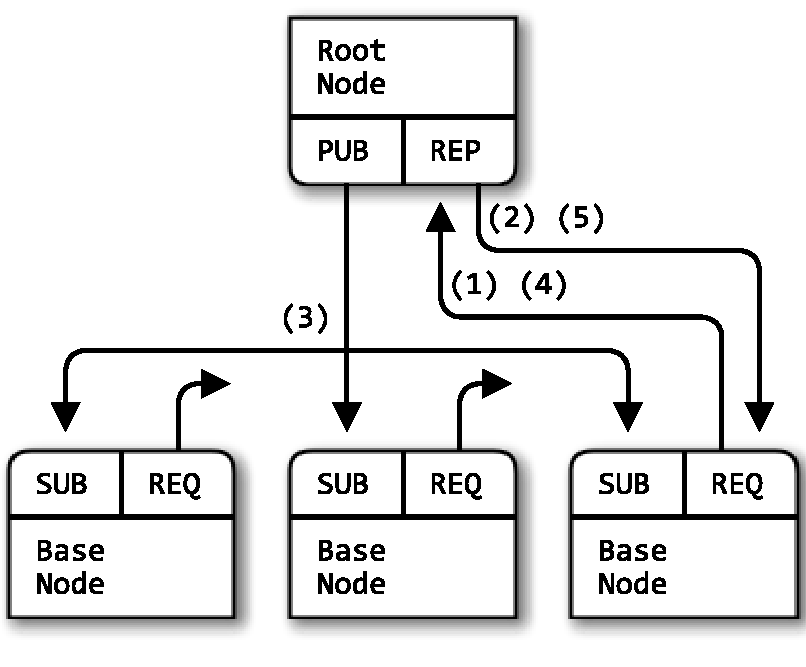
\includegraphics[scale=0.5]{branch-recovery.pdf}
    \label{fig:proto_branch_reco_image}
    \caption[Branch Recovery Protocol Diagram]
	    {Branch Recovery Protocol Diagram: (1) \textit{Metric} nodes send \texttt{SOS} requests, (2) \textit{Root}
	     replies with \texttt{KEEPCALM}, (3) \textit{Root} sends \texttt{GROUP} only to nodes in branch, (4)
	     \textit{Metric} nodes send \texttt{POLO} requests, (5) \textit{Root} replies with \texttt{STOP}}
\end{figure}

\texttt{SOS} and \texttt{KEEPCALM} are shorthand for the \texttt{CONTROL} message with a command value of \texttt{"sos"}
and \texttt{"keepcalm"} respectively. The \texttt{POLO} and \texttt{STOP} messages come directly from the Topology
Protocol.

The \texttt{GROUP} message is similarly shorthand for the \texttt{TOPO} message with a key value of
\texttt{"/GROUP/<group-name>"}. This takes advantage of ZeroMQ's Pub-Sub filtering to only stop the faulty branch.

\begin{figure}[H]
\vspace{+10pt}
\begin{verbatim}
root-recovery  = *election
election       = C-WUTUP *C-YO C-IWIN
\end{verbatim}
\vspace{-5pt}
\caption[Root Recovery Protocol]
        {Root Recovery Protocol: \texttt{C-} represents a \textit{Collector} node sending a message.}
\label{fig:proto_reco_root_spec}
\end{figure}

As each \textit{Collector} node detects the \textit{Root} node has died, it attempts to start an election via the
\texttt{WUTUP} message. \textit{Collector} nodes with higher UUIDs will respond to the first \textit{Collector} by
sending the \texttt{YO} message. If no \texttt{YO} messages are received by the first \textit{Collector}, the
\texttt{IWIN} message is sent out to all \textit{Collector} nodes, self-declaring the first \textit{Collector} as the
new Root.

\begin{figure}[H]
    \centering
    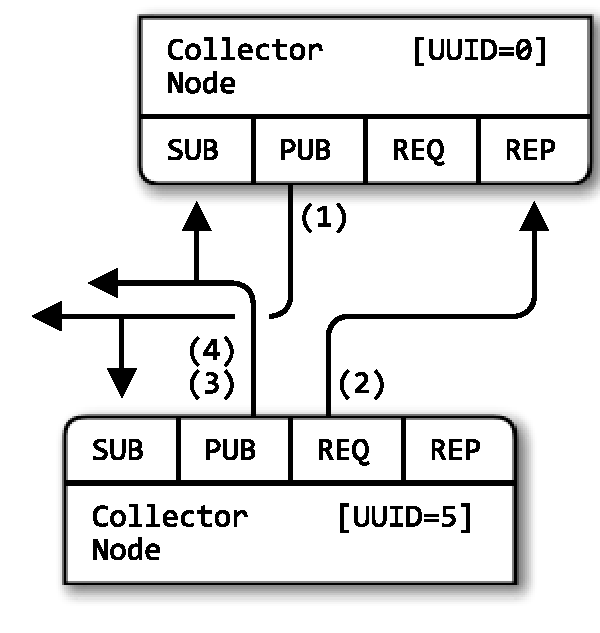
\includegraphics[scale=0.5]{root-recovery.pdf}
    \label{fig:proto_root_reco_image}
    \caption[Root Recovery Protocol Diagram]
	    {Root Recovery Protocol Diagram: (1) \texttt{WUTUP}, (2) \texttt{YO}, (3) \texttt{WUTUP}, (4) \texttt{IWIN}}
\end{figure}

The \texttt{WUTUP} and \texttt{IWIN} messages are shorthand for \texttt{TOPO(key="/RECOVERY/wutup"} and
\texttt{TOPO(key="/RECOVERY/iwin"} respectively. The \texttt{YO} message is shorthand for
\texttt{CONTROL(command="yo")}.



\chapter{Analysis}
\label{analysis}

To verify \dcamp meets both the transparency and scalability distributed performance framework criterion outlined in
Chapter \ref{introduction}, several experiments were run on an installation of \dcamp in a test environment. The goal of
these experiments was two fold: measure \dcamp's transparency in a real-world environment as well as determine the
thresholds for several key configuration parameters as \dcamp scales.

Any DPF can be configured in such a way that it impacts the performance of the system being monitored, for example by
collecting and reporting every available global metric and per-process metrics at the fastest sampling period.
Therefore, it is necessary for the system administrator to know what reasonable configuration values should be used to
monitor a given distributed system.

Likewise, for \dcamp to scale, it is important for the number of child nodes per parent to be limited to a reasonable
number. These experiments help to define ``reasonable'' for various scenarios, environments, and performance monitoring
requirements.

\section{Transparency}

To measure the impact of \dcamp on a monitored process, a workload is defined and measured with and without \dcamp
active. The measured difference in performance of the monitored process is defined to be \dcamp's monitoring overhead.

\subsection{Workload}

Apache JMeter\cite{jmeter} (v2.11) is used to run load against a default-configured Apache instance on a Lenovo Thinkpad
(dual 2.16GHz Centrino Duo T2600, 2GB 667MHz DDR2, SATA) running Ubuntu 13.10. The client machine, a MacBook Pro (2.7GHz
Core i7, 8GB 1333MHz DDR3, SSD) running OSX 10.9, is directly connected to the Apache server via crossover gigabit
Ethernet.

Each test run includes 18 different load points, scaling the number of client threads from 2 to 2048. For every load
point, the threads continuously (in this order)

\begin{enumerate}
\item load a static home page,
\item load a PHP page which calculates the 25th Fibonacci number (see Figure \ref{fig:fib25_list}), and
\item download a 5MB file of random binary data.
\end{enumerate}

The 25th Fibonacci workload is CPU-bound, and the 5MB download is disk-bound; the home page workload is only used to
seed the client connection and is not part of the analysis measurements. After the ramp up phase of each load point
(launching 10 threads per second), the test ensures all threads continue to execute simultaneously for five minutes
before shutting down.

The arithmetic mean of the request latency for each step at each load point is then calculated and averaged across three
distinct runs of the same test.

\begin{figure}[H]
\vspace{+10pt}
\begin{lstlisting}[language=php,frame=single,basicstyle=\footnotesize\ttfamily]
<?php
function F($n) {
    if ($n == 0) { return 0; }
    if ($n == 1) { return 1; }
    return F($n - 1) + F($n - 2);
}
?>
<html>
  <body>The 25th Fibonacci number is <?= F(25) ?>.</body>
</html>
\end{lstlisting}
\vspace{-10pt}
\caption[Recursive 25th Fibonacci PHP Script]
	{Recursive 25th Fibonacci PHP Script: A naive approach was used in the implementation of \texttt{F()} in order
	 to put more load on the server CPU.}
\label{fig:fib25_list}
\end{figure}

\subsection{\dcamp Configuration}

Each \dcamp configuration level monitors four global metrics and three process-specific metrics on the Apache
process(es). The global metrics are CPU usage (\texttt{proc}), memory usage (\texttt{mem}), disk throughput
(\texttt{disk}), and network throughput (\texttt{net}); the Apache metrics are CPU usage (\texttt{apache\_cpu}), memory
usage (\texttt{apache\_mem}), and combined disk/network throughput (\texttt{apache\_io}). Below are the various sample
periods used for the transparency test runs.

\begin{itemize}
\item \textbf{baseline} -- \dcamp off
\item \textbf{5m} -- all metrics every 300 seconds, heartbeats every 60 seconds
\item \textbf{1m} -- all metrics every 60 seconds, heartbeats every 60 seconds
\item \textbf{10s} -- global metrics every 300 seconds, Apache metrics every 10 seconds, heartbeats every 300 seconds
\item \textbf{1s} -- global metrics every 300 seconds, Apache metrics every 1 second, heartbeats every 300 seconds
\end{itemize}

No thresholds were defined for any of the above configurations. That is, Sensor nodes immediately reported every sample
instead of holding them for later reporting.

\subsection{Results}

In the CPU-bound Fibonacci test, the biggest relative increase in request latency occurs between the runs with two and
four threads. This correlates to the two physical CPU cores on the system exceeding capacity. The 1m config run exhibits
the worst performance of all the CPU-bound tests. This shows that global metric monitoring is actually more CPU
intensive than collecting per-process metrics, even for processes with many active processes.

The rate at which request latency worsens begins to level off starting at the 512 thread load point. This is also the
load point at which Apache begins to return errors. As the percentage of requests resulting in errors increases, the
latency of the successful requests improves slightly. This explains the trend line shift.

\begin{figure}[H]
    \centering
    \vspace{-20pt}
    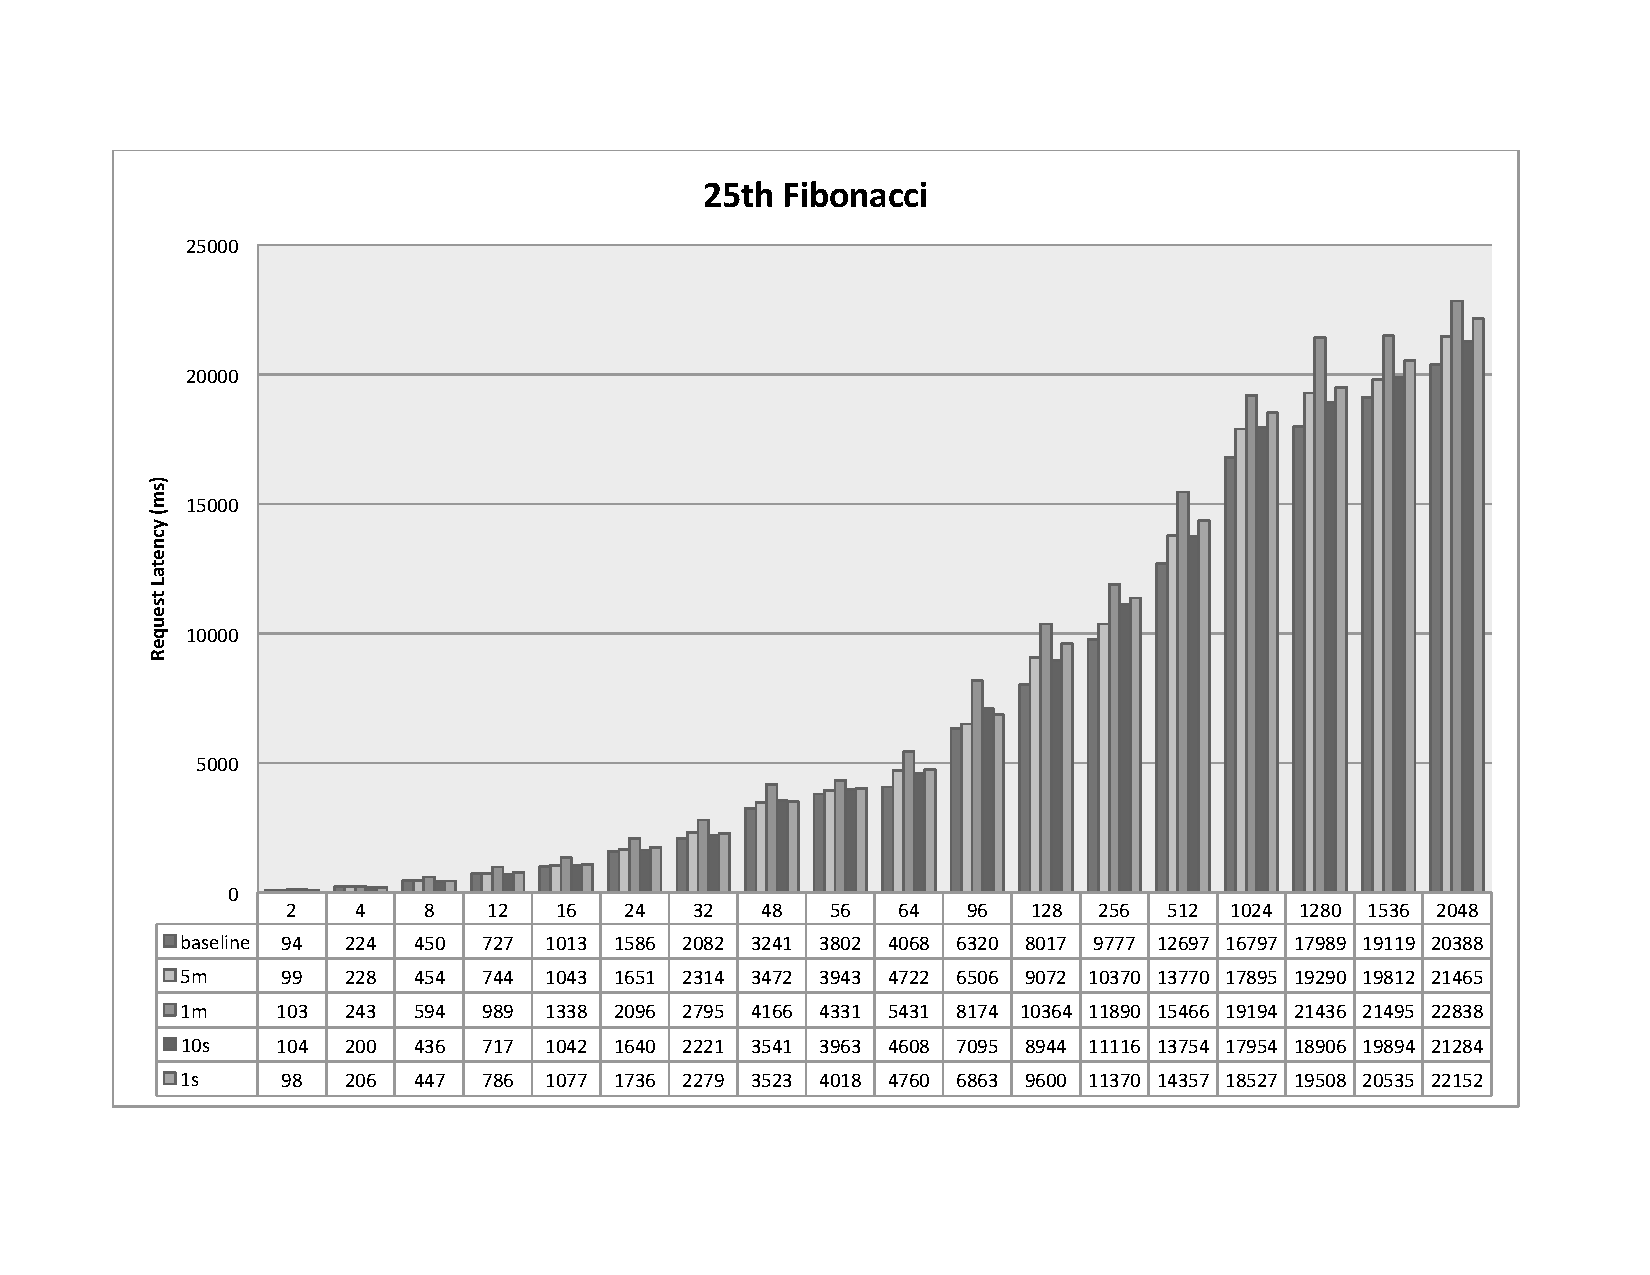
\includegraphics[scale=0.5]{compare-fib.pdf}
    \vspace{-50pt}
    \caption{25th Fibonacci Results}
    \label{fig:fib25_graph}
\end{figure}

Apache's disk-bound performance measured in the 5MB download test is relatively unaffected by \dcamp. This graph also
shows the 512 thread load point as the beginning of a trend line shift, again correlating with the increase in request
error rate.

\begin{figure}[H]
    \centering
    \vspace{-20pt}
    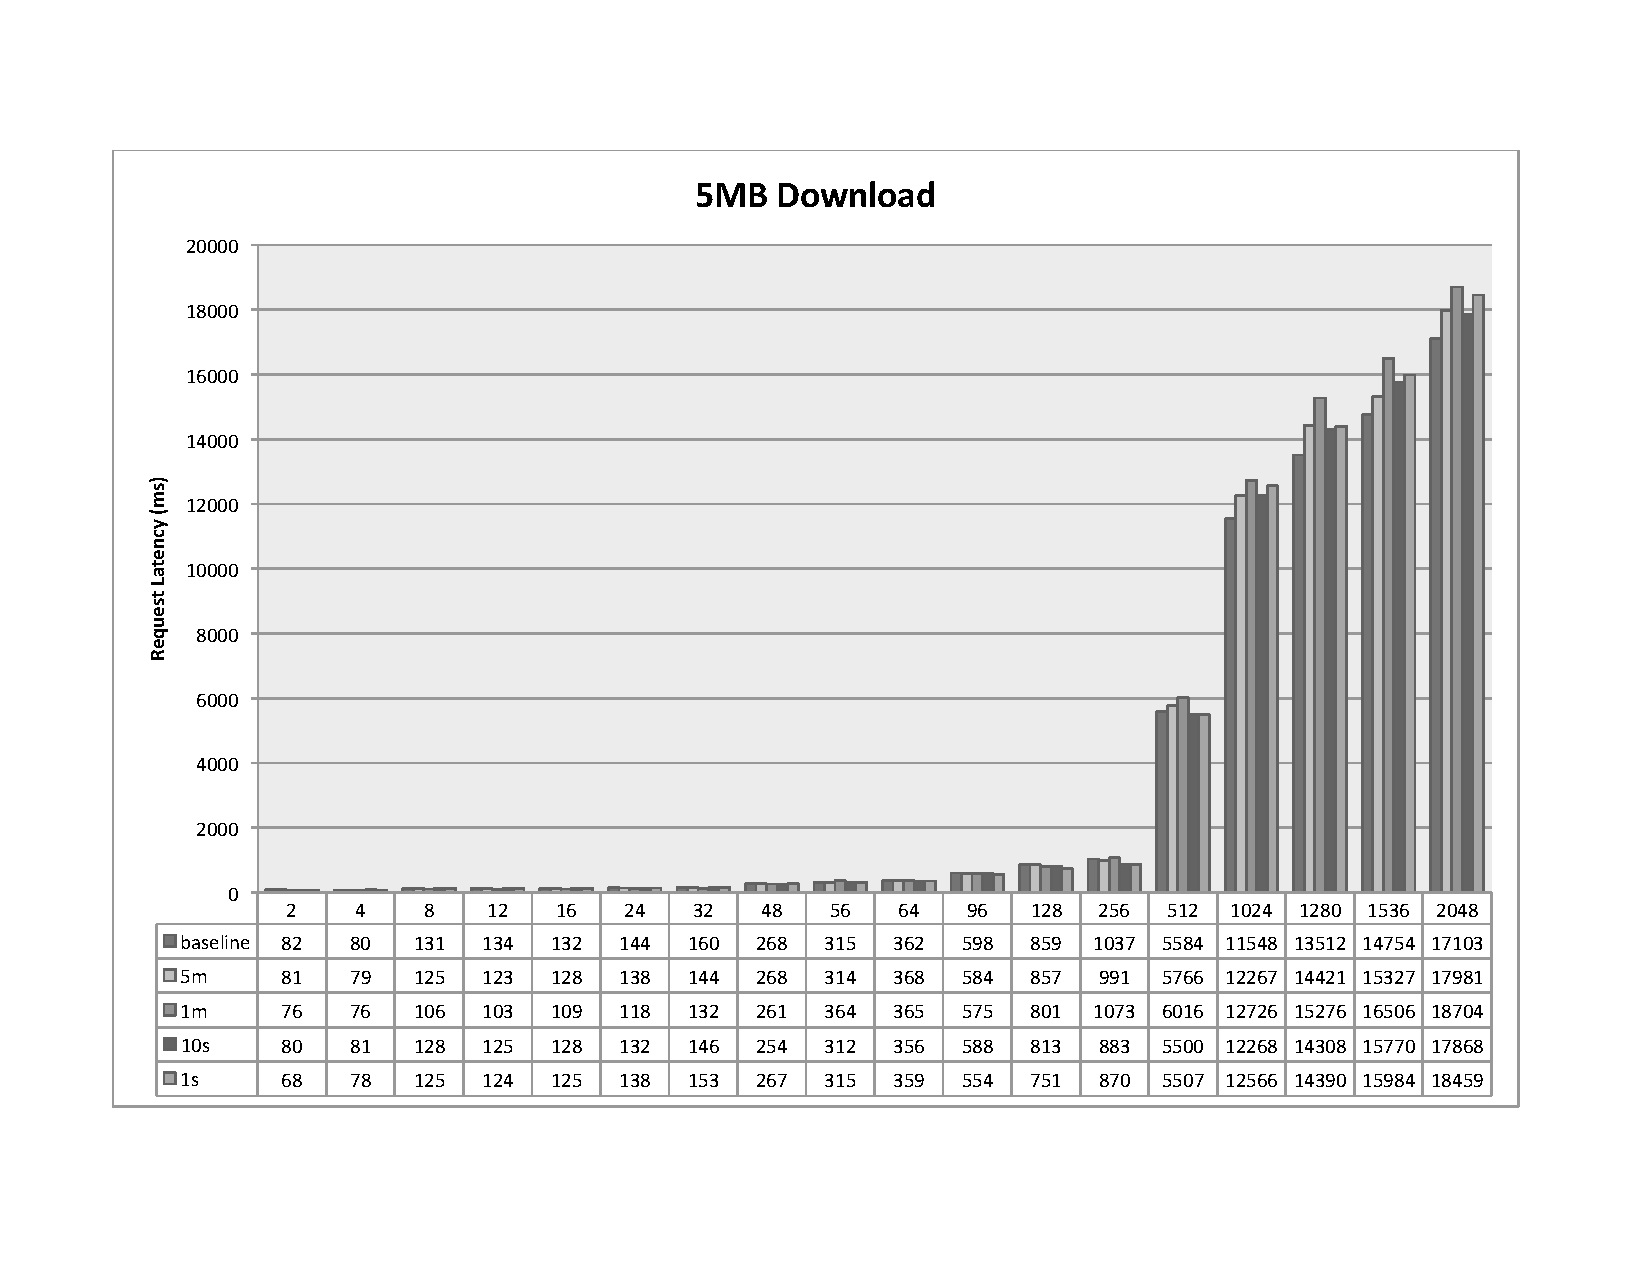
\includegraphics[scale=0.5]{compare-down.pdf}
    \vspace{-50pt}
    \caption{5MB Download Results}
    \label{fig:down5mb_graph}
\end{figure}

A few observations can be drawn from these results.

When nodes are not expected to fail frequently, using longer heartbeat periods reduces the impact \dcamp has on the
system. It is better to monitor a process using a faster sample period than an entire system using a slower sample
period. The \dcamp system impact is noticeable but a considerably smaller factor than the impact hardware limitations
have on performance monitoring.

\section{Scalability}

One of the primary measures of scalability for a distributed system is its network traffic.\cite{zanikolas2005} By
simulating successively larger \dcamp systems (with respect to node count), once can extrapolate \dcamp's effectiveness
at monitoring large distributed systems and how to best configure its metric collections.

\subsection{Workload}

\dcamp is setup to monitor a machine's global metrics, scaling the number of simulated nodes in the \dcamp system from
three nodes (one Root, one Collector, one Sensor) up to 200 nodes (eight groups with twenty-five nodes per group). The
metric configuration is kept constant for each test run. As \dcamp starts, monitors in steady state, and shuts down, the
machine's network traffic is monitored and recorded every five seconds.

The test machine is a MacBook Pro (2.7GHz Core i7, 8GB 1333MHz DDR3, SSD) running OSX 10.9. All simulated \dcamp nodes
use endpoints on the machine's loopback interface, and only the loopback interface traffic is monitored. The machine is
otherwise entirely idle during the test runs.

\subsection{\dcamp Configuration}

\dcamp is configured to monitor and report the below global metrics, using a heartbeat of 60 seconds.

\begin{itemize}
\item CPU usage every 60 seconds
\item total disk throughput every 120 seconds
\item total network throughput every 120 seconds
\item memory usage every 60 seconds
\end{itemize}

No thresholds were defined for the above configuration. That is, Sensor nodes immediately reported every sample instead
of holding them for later reporting.

\subsection{Results}

Sparklines of each load point show the same pattern: highest network traffic occurs during start up and then also on
shutdown. This pattern follows the design of \dcamp which uses a chatty configuration protocol and a terse data
protocol. The rest of steady operation shows expected low network traffic except on sample periods.

\begin{figure}[H]
    \centering
    \vspace{-20pt}
    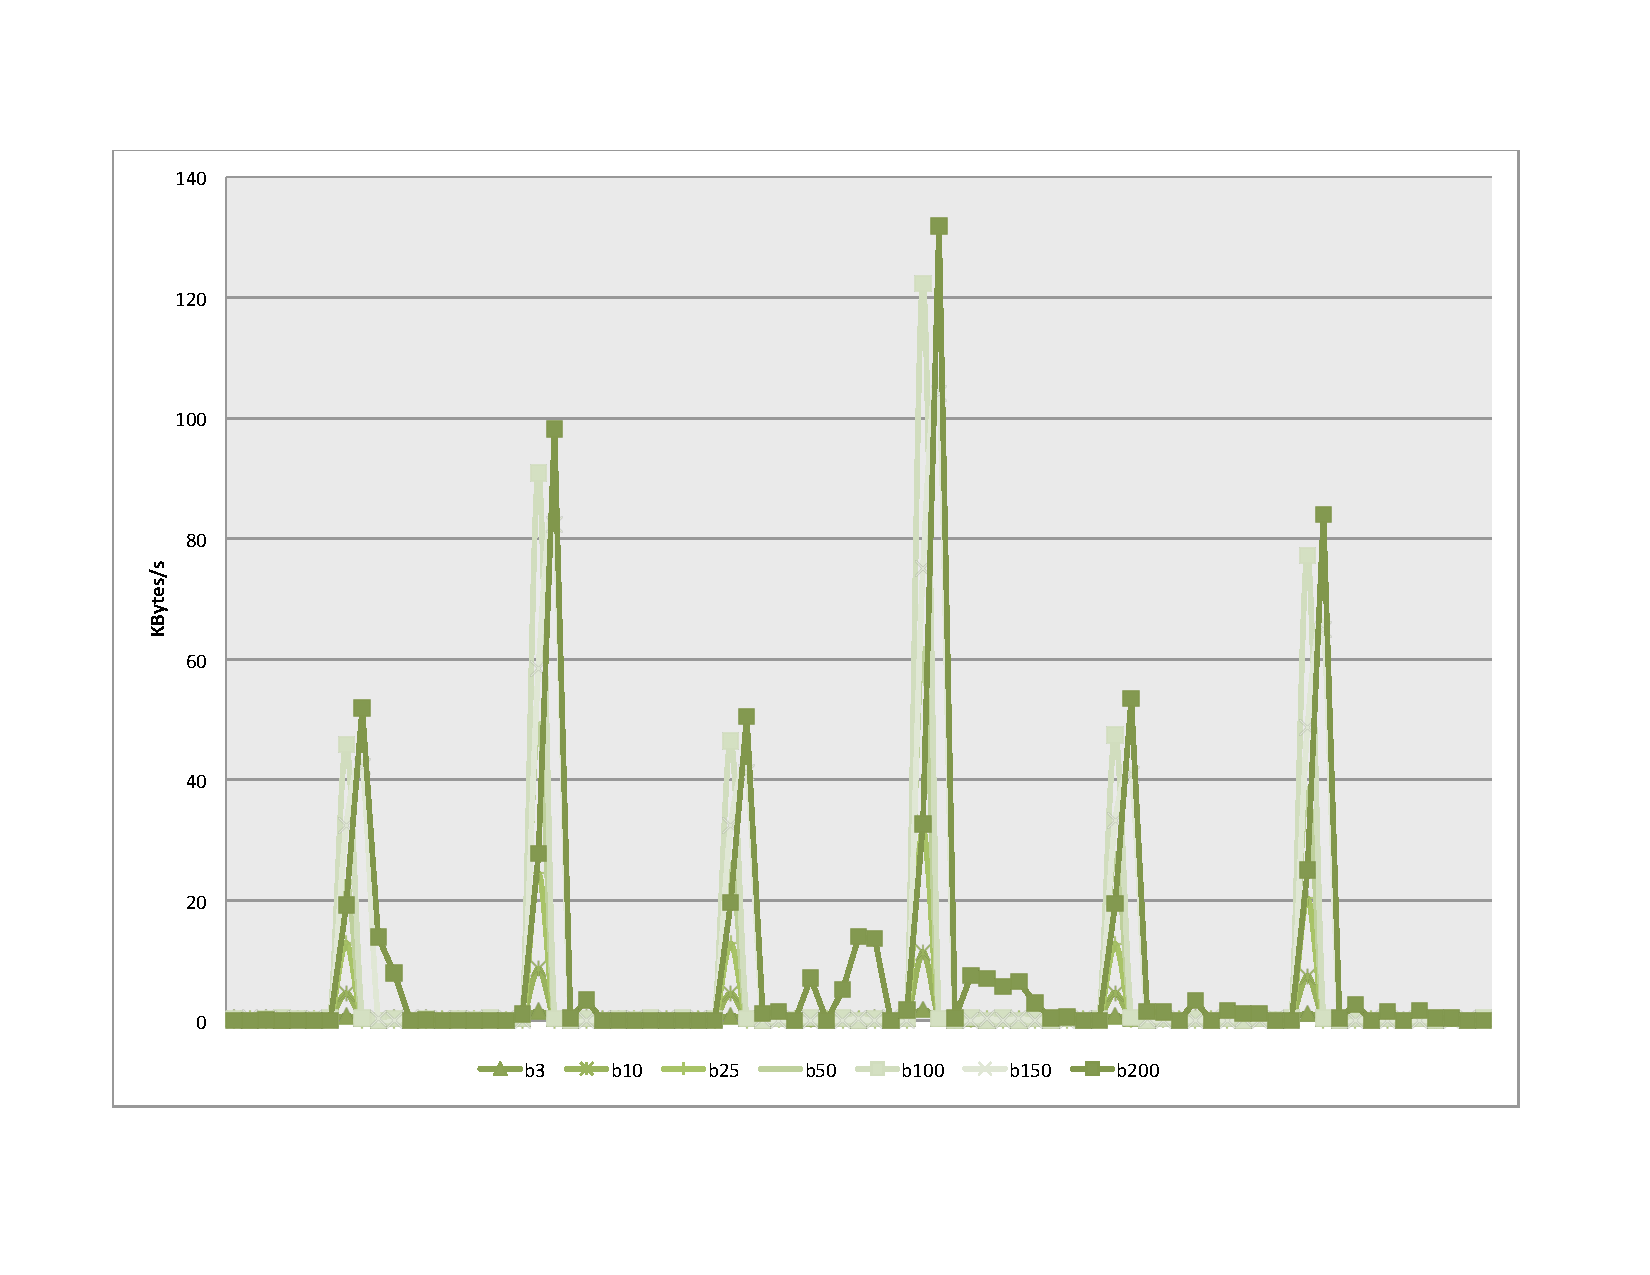
\includegraphics[scale=0.5]{dcamp-net-bytes-steady.pdf}
    \vspace{-40pt}
    \caption{Network bytes during steady operation as the number of \dcamp nodes increases.}
    \label{fig:net_bytes_steady_graph}
\end{figure}

\begin{figure}[H]
    \centering
    \vspace{-20pt}
    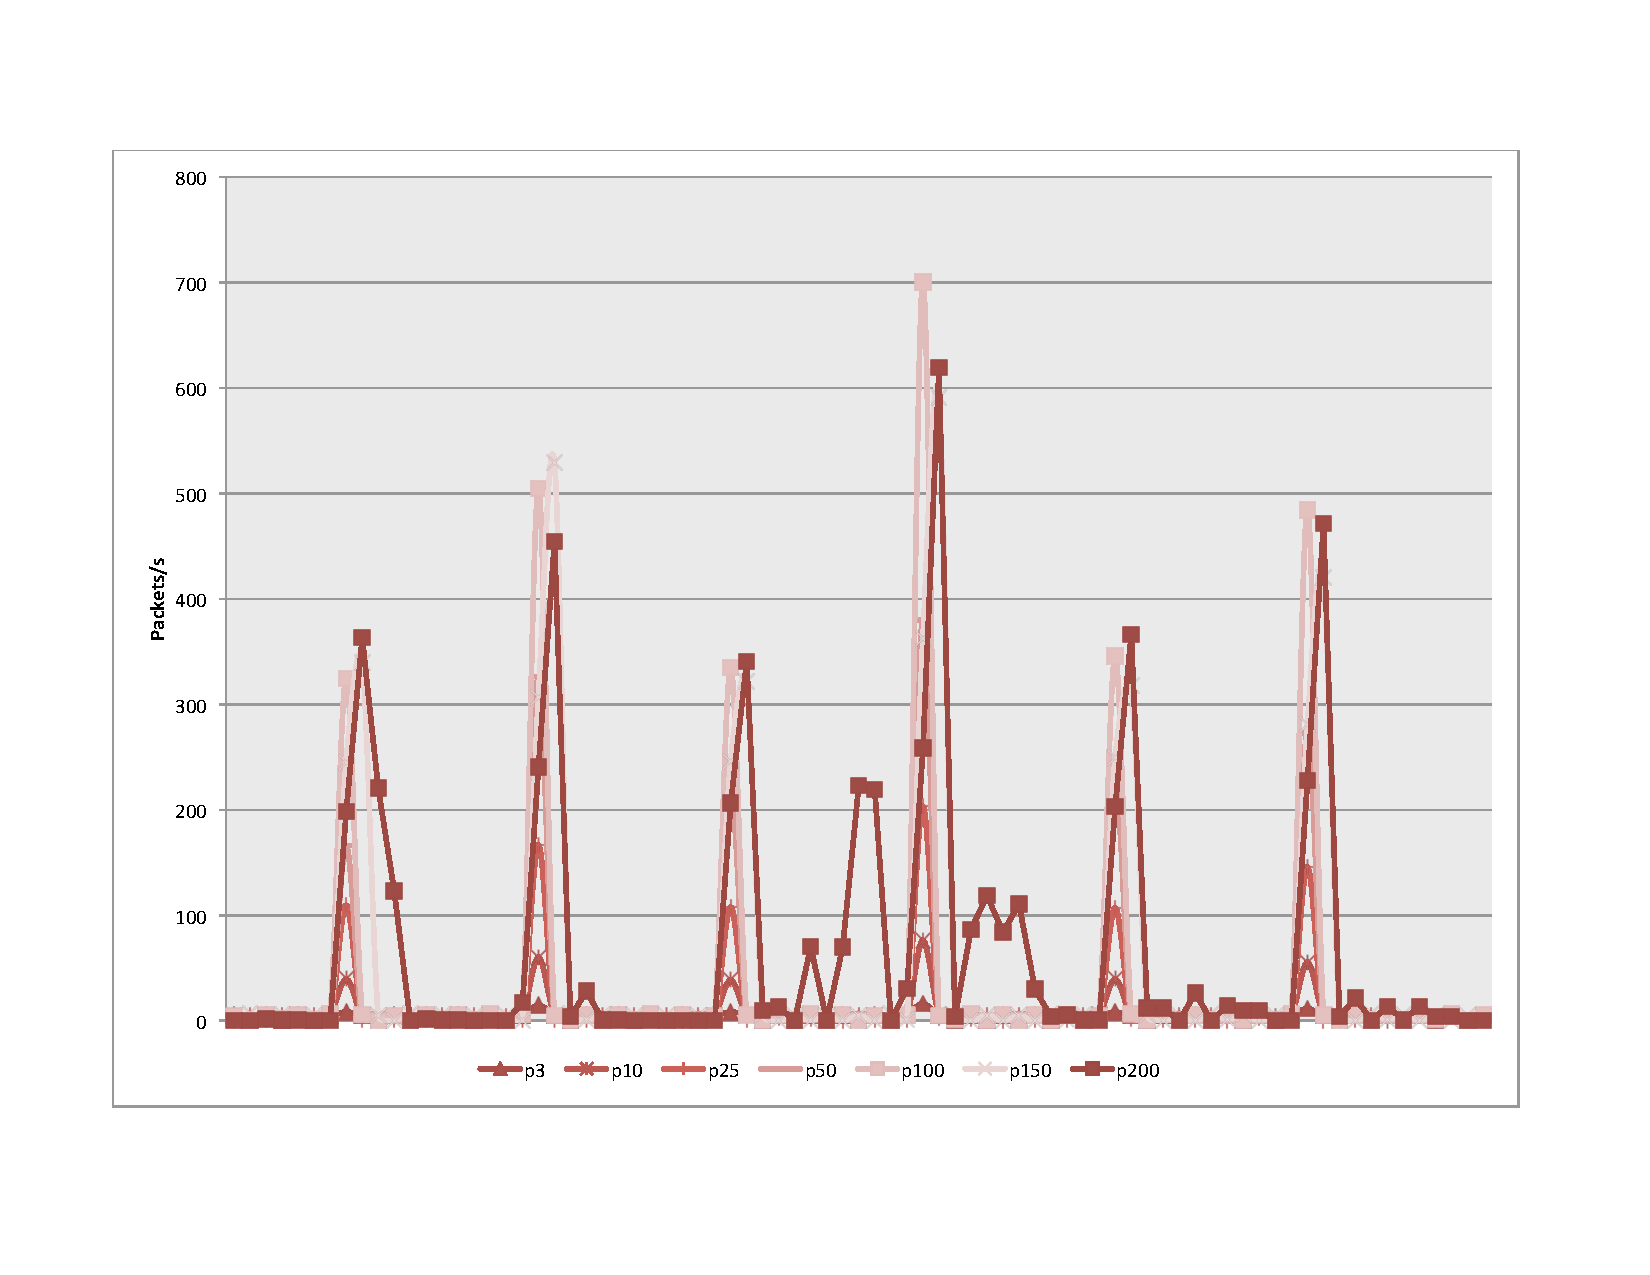
\includegraphics[scale=0.5]{dcamp-net-packets-steady.pdf}
    \vspace{-40pt}
    \caption{Network packets during steady operation as the number of \dcamp nodes increases.}
    \label{fig:net_packets_steady_graph}
\end{figure}

As the node count increases, the rate at which bytes/packets are sent and received increases. This correlates with the
larger configuration which \dcamp must track as well as the additional nodes sending and receiving data. Looking at the
same values but also relating them to the number of nodes in the system, one sees the configuration size grows faster
than the number of nodes.

However, the number of messages being sent per node actually goes down and levels off just under 1 packet per node per
second. This can be attributed to the fact that the number of Sensor nodes increases faster in relation to the number of
Collector nodes. That is, Sensor nodes do not require full-configuration replication and send/receive fewer messages
since they are relatively uninvolved with topology coordination in comparison to Collector nodes.

As this ratio increases, it is expected the number of messages per node to decrease. This latter observation indicates a
higher number of child nodes per parent would result in lower network utilization and better \dcamp scalability.

\begin{figure}[H]
    \centering
    \vspace{-20pt}
    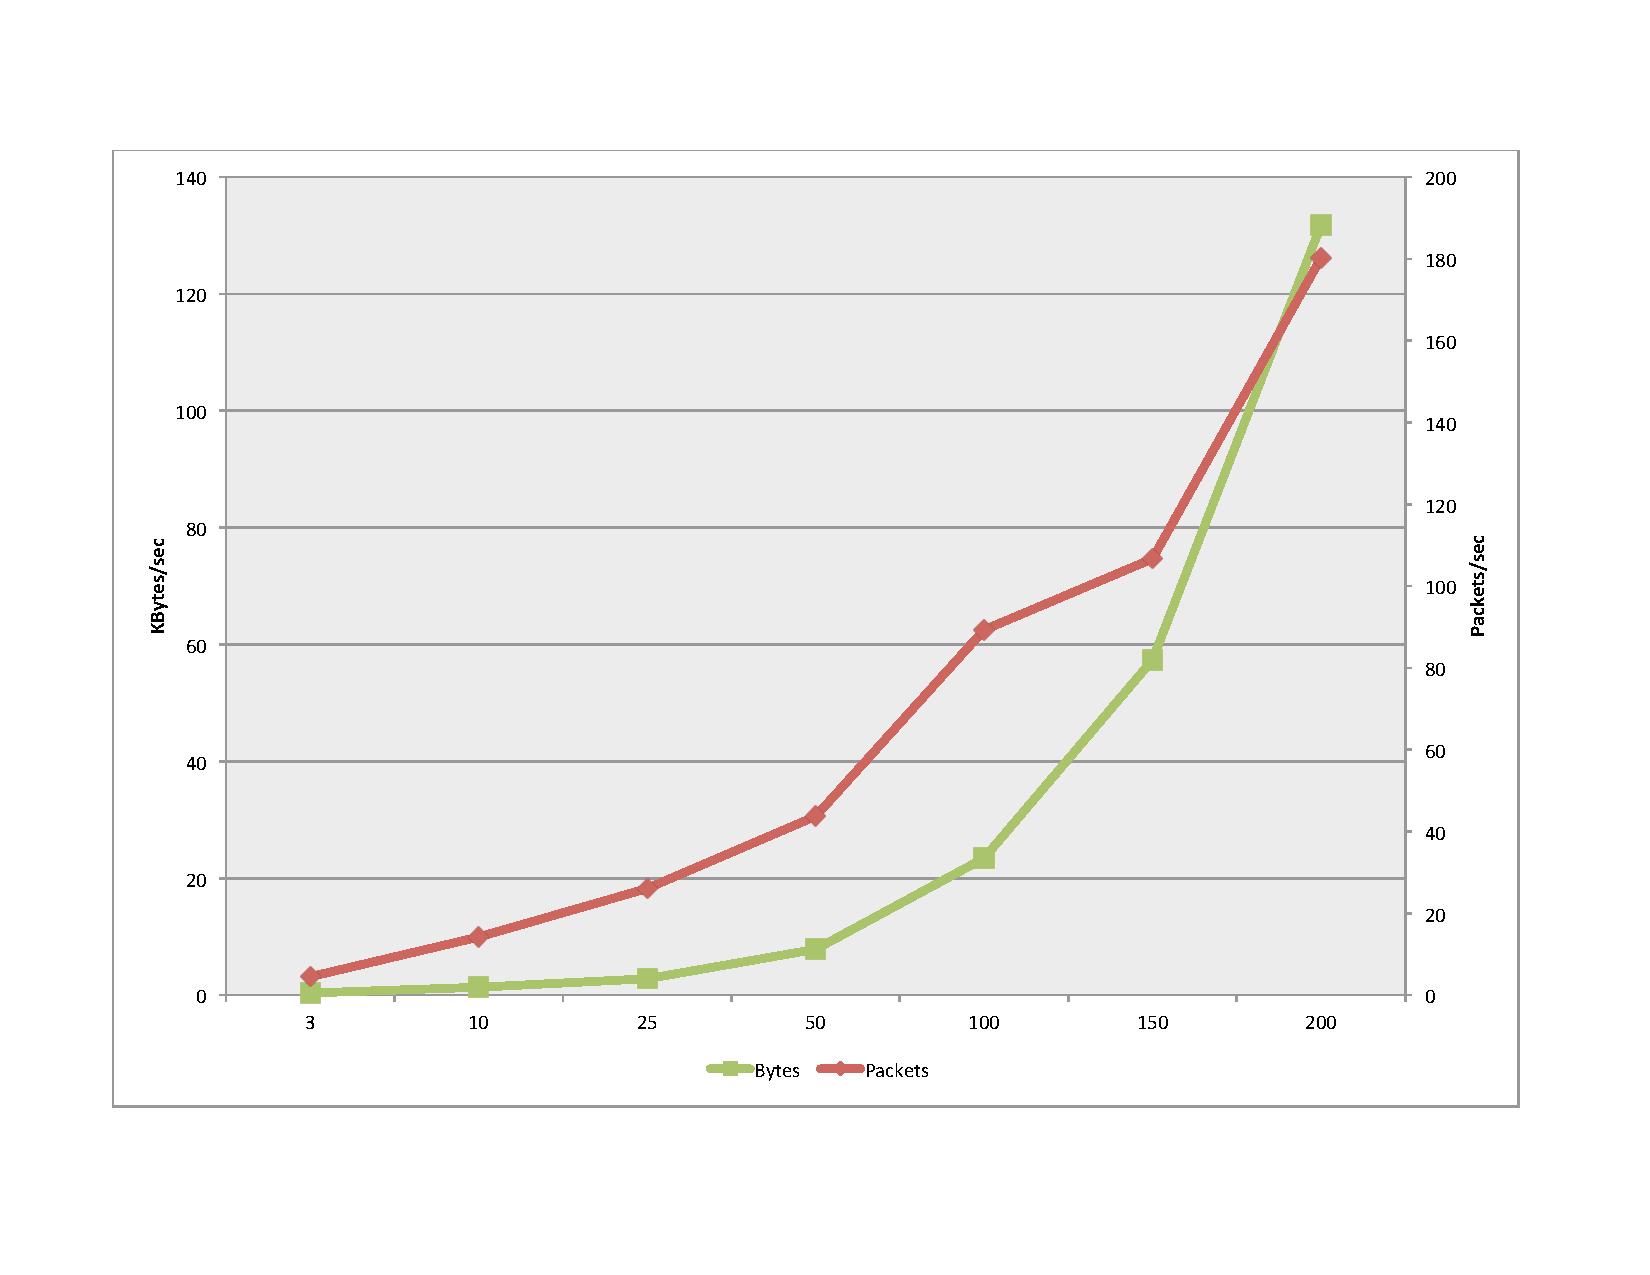
\includegraphics[scale=0.5]{dcamp-net-average.pdf}
    \vspace{-40pt}
    \caption{Average Bytes/Packets as the number of \dcamp nodes increases.}
    \label{fig:net_avg_graph}
\end{figure}

\begin{figure}[H]
    \centering
    \vspace{-20pt}
    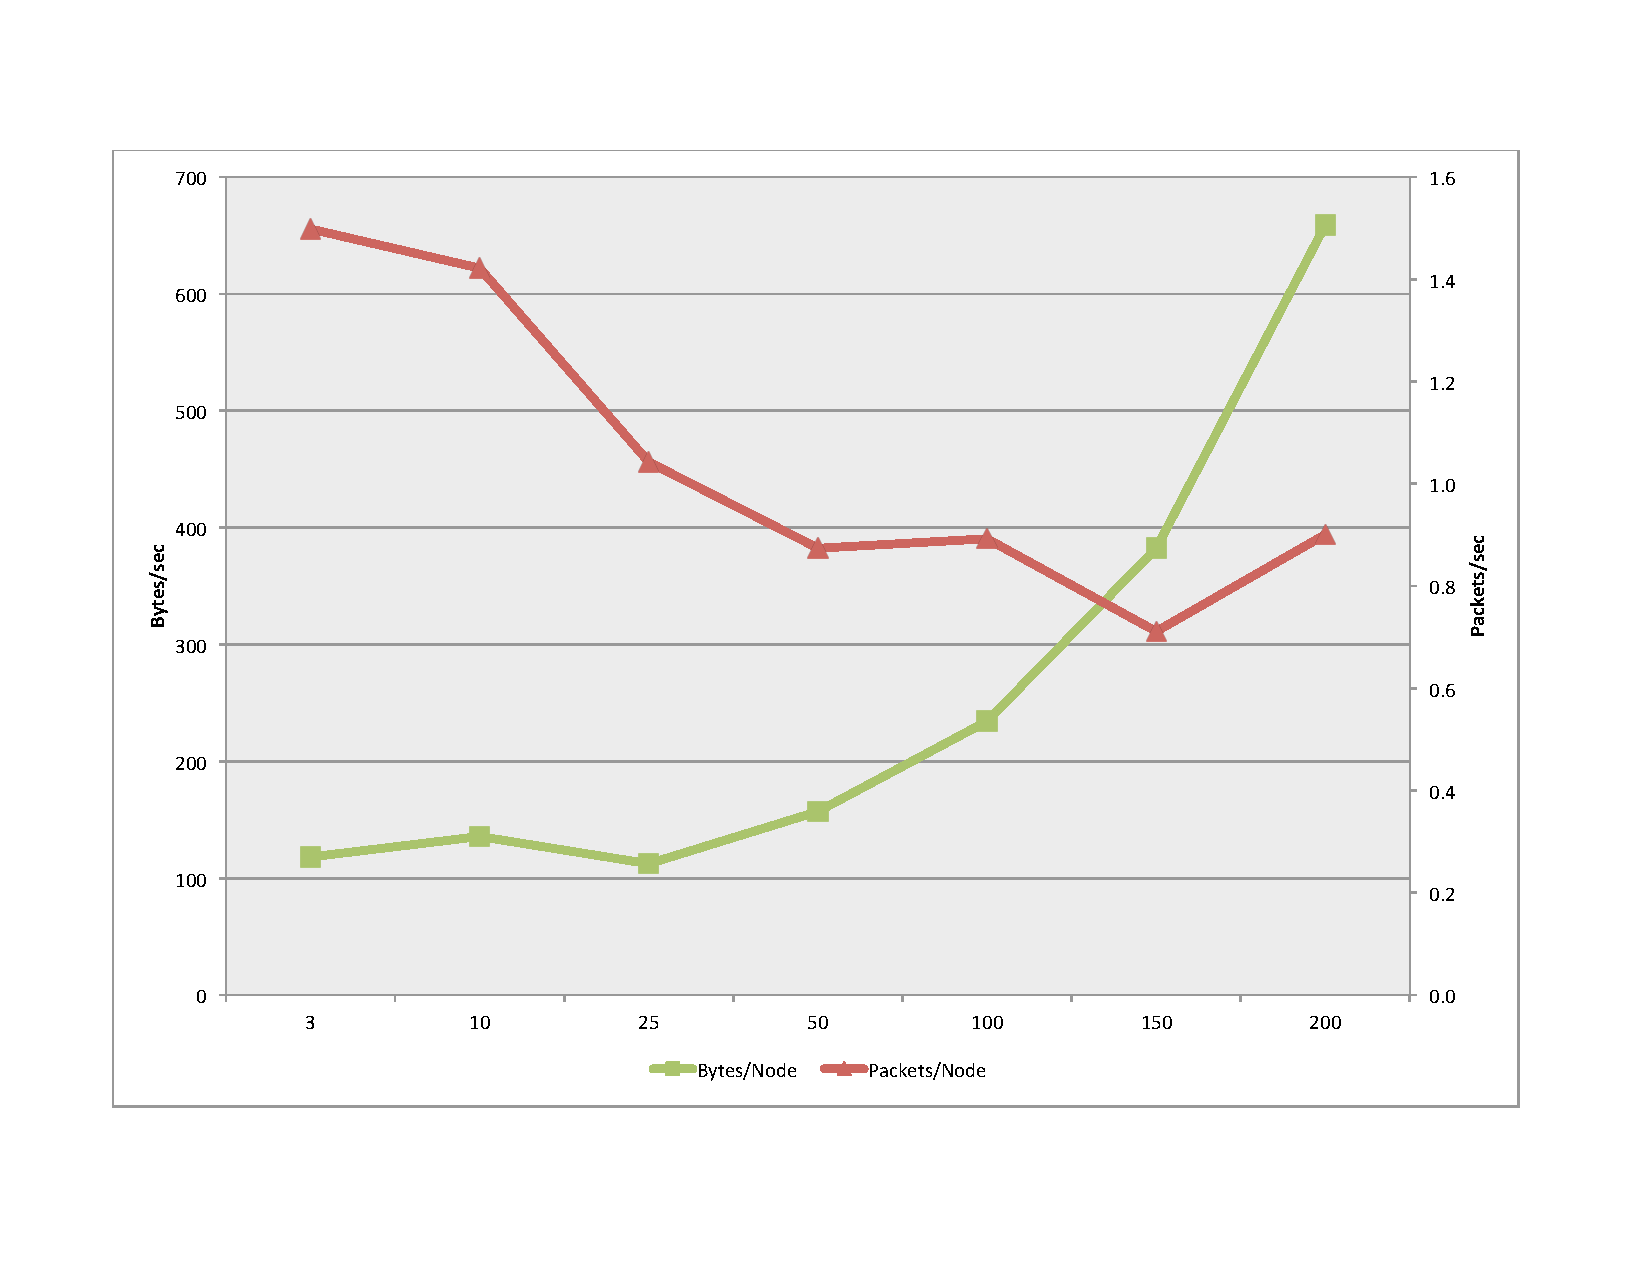
\includegraphics[scale=0.5]{dcamp-net-average-pernode.pdf}
    \vspace{-40pt}
    \caption{Average Bytes/Packets Per Node as the number of \dcamp nodes increases.}
    \label{fig:net_avg_pernode_graph}
\end{figure}

\chapter{Related Work}
\label{related_work}

\emph{THIS SECTION IS FROM MY 508 PAPER \newline AND NEEDS TO BE CLEANED UP}

Being distributed, a framework must collect data from a large number of nodes and aggregate the data to one node or client.
Implementations have been built using centralized, hierarchical, peer-to-peer and any number of other architectures.
There are three types of metric gathering techniques: (1) hardware counters and sensors use specialized hardware to gather highly accurate metrics and are highly dependent on the underlying hardware architecture, (2) software sensors use modern operating system interfaces to acquire moderately accurate performance metrics in an architecture-independent interface, and (3) hybrid approaches use a combination of hardware and software sensors to attain a balance between the two.

There are a number of distributed performance frameworks being actively researched and developed, both academically and commercially.
This work defines a set of criteria for evaluating distributed performance frameworks to measure the usefulness and viability of the framework.
In the next section I list similar survey work, showing the novelty of this paper.
Section 3 presents the evaluation criteria, section 4 provides the evaluation results of several distributed performance frameworks, and section 5 concludes.

\section{Related Work}
Several papers have been published dealing with this topic and which try to give an overview of the current state of distributed performance frameworks.
This work, while related, differs in two main aspects: (1) the evaluation criteria presented here is more complete than previous works' requirements and (2) this work looks specifically at distributed performance frameworks rather than distributed system or grid tools and frameworks.

Zoraja et al. include a section on Monitoring Issues in their work on \newline OMIS/OCM, CORAL, and MIMO \cite{zoraja1999} focusing on design and implementation issues for monitoring systems.
These monitoring issues share some critical points with the criteria presented here, but the work lacks an analysis of other distributed performance frameworks and only includes limited analysis of the presented frameworks against the listed monitoring issues.
\cite{hofmann1994} provides a short survey of related monitoring systems in comparison to the ZM4/SIMPLE monitoring environment.
While this survey does look at a number of important framework characteristics, it is restricted to hybrid distributed performance frameworks.

Allan and Ashworth published an exhaustive survey of distributed computing tools \cite{allan2001} but did not present any particular focus on distributed performance frameworks nor did they include a set of criteria for evaluating frameworks.
Zanikolas et al. present an in-depth taxonomy of grid monitoring systems \cite{zanikolas2005}, including a set of general requirements for monitoring systems.
Their work does much for defining a good set of criteria for evaluating and analyzing distributed performance frameworks, but has a much broader scope than this work.
This work expands on their monitoring system requirements to account for the completeness and validity of distributed performance frameworks.

\section{Analysis Results}
The distributed performance frameworks analyzed in this section were chosen based on their categorization in the \cite{zanikolas2005} taxonomy; only level 2 frameworks are included.
Level 2 frameworks are defined as having at least one type of republisher in addition to producers; these frameworks usually distribute functionality across multiple hosts. \cite{zanikolas2005}
A limited analysis is conducted by reviewing the available literature, and further analysis (i.e., verifying scalability, transparency, and validity) is left as future work.

\subsection{NetLogger}
Work done by Brian Tierney and Dan Gunter \cite{tierney1998} \cite{gunter2000} presents the Network Application Logger Toolkit (NetLogger).
This framework can be used to monitor the performance of distributed systems at a very detailed level.
With a new logging format and activation service \cite{gunter2002} the authors improved upon their previous work and increased the toolkit's scalability and data delivery models.
NetLogger is being actively developed and is one of the more well known distributed performance frameworks.
The toolkit is composed of four parts: an API and library for instrumenting a given application, a set of tools for collecting and sorting logs, performance sensors, and a visualization user interface for the log files.

Each part assumes the system clocks of the individual nodes are accurate and synchronized (the authors mention the use of NTP to achieve a required clock synchronization of one millisecond).
The instrumentation of code allows NetLogger to gather more detailed data from an application-to-application communication path, such as traces of network packets through a call hierarchy.
The instrumentation also allows the activation service to update the monitoring of parts of the system dynamically as consumers subscribe to various events and metrics.

Their research has shown NetLogger to be highly scalable, complete, and transparent as well as valid.
The activation service provides a push data delivery and can utilize the security mechanisms part of current web services in order to authenticate requests for performance data.
NetLogger is currently implemented for C, C++, Java, Perl, and Python applications.
Because the framework lacks black box characteristics, its portability is greatly reduced.

\subsection{JAMM}
Java Agents for Monitoring and Management (JAMM) \cite{tierney2000} is the fruit of work by the authors of NetLogger to build a monitoring system with managed sensors. 

The JAMM system consists of six components: sensors, sensor managers, event gateways, directory service, event consumers, and event archives.
There is a sensor manager on each host, with the sensors acting as producers for the gateways which they publish the data to.
The gateways can then filter and aggregate the incoming data according to consumer queries.
The directory service is used to publish the location of the sensors and gateways, allowing for dynamic discovery of active sensors by the consumers.
The event archive is used for historical analysis purposes.

JAMM explicitly uses a pull data delivery model where data is only sent when requested by a consumer.
The overall architecture is generally distributed with the directory service being centralized.
JAMM, being heavily based off of NetLogger, inherits the validity, completeness, security, and transparency of NetLogger along with its lack of portability.
JAMM does, however, prove itself in terms of scalability with it's own architecture.

\subsection{Hawkeye}
Hawkeye \cite{hawkeye} is a monitoring and management tool for distributed systems which makes use of technology previously researched and developed as part of the Condor project \cite{litzkow1988}.
Condor provides mechanisms for collecting information about large distributed computer systems.
Hawkeye is being readily developed and is freely available for download on Linux and Solaris.

Hawkeye uses a general push delivery model by configuring Condor to execute programs, or modules, at given time intervals, collect performance data, and send it to the central manager.
These modules are configurable such that the "period' of module execution can be set to a given time frame in seconds, minutes, or hours or the module can be executed in "continuous" mode where the module's execution never ends.
The available modules for monitoring a Condor pool include: disk space, memory used, network errors, open files, CPU monitoring, system load, users, Condor Node, Condor Pool, and Grid Probe.
Custom modules can also be developed and installed for monitoring of arbitrary resources and metrics.
Data can be accessed from the central manager via an API, CLI, or GUI.

While no experiments have been run, the generally centralized manager reduces the Hawkeye framework's scalability, and its transparency is unknown.
The frameworks module based producer architecture gives it an infinite completeness, but being only available on Linux and Solaris makes the framework less portable.
Lastly, the ability to run jobs securely on target machines has been left as future work by the authors.

\subsection{SCALEA-G}
Truong and Fahringer present SCALEA-G \cite{truong2004}, an unified monitoring and performance analysis system for distributed systems.
It is based on the Open Grid Service Architecture \cite{foster2002} and allows for a number of services to monitor both grid resources and grid application.
SCALEA-G uses dynamic instrumentation to profile and trace Java and C/C++ applications in both push and pull data delivery models, making the framework both scalable and portable.

The SCALEA-G framework is composed of several services: directory service, archival service, sensor manager service, instrumentation service, client service, and user portal.
These services provide the following functionality respectively: publishing and searching of producers and consumers, storage of performance results, management of sensors, dynamic instrumentation of source code, administering clients and analyzing data, and on-line monitoring and performance analysis.

The framework makes use of secure sockets to achieve secure communications and achieves high completeness via code instrumentation.
Unfortunately, the authors do not provide any report on SCALEA-G's validity or transparency.

\subsection{IMPuLSE}
Integrated Monitoring and Profiling for Large Scale Environments \cite{bridges2004} was designed to address "operating system-induced performance anomalies" and provide "accurate, low-overhead, whole-system monitoring." The authors have chosen to develop a message-centric approach which associates data with messages rather than hosts and a system-wide statistical sampling to increases the framework's scalability.

The IMPuLSE framework is still in the design stage, and therefore lacks any implementation data outside of their new message-centric design pattern which shows promising results.
Unfortunately, this leaves the framework with unknown transparency, security, completeness, portability, and validity.

\section{Conclusion}
There are a number of high quality and effective distributed performance frameworks being actively researched and developed, but with some frameworks having more research than others, there is a natural disparity of information about each framework.
While the frameworks vary in distributed architecture and features, they all fulfill the minimum requirements of performance frameworks.
The frameworks analyzed in this work are mainly software based sensor frameworks.
This was chosen due to the inherent portability advantage of software sensors over hardware or hybrid sensors.

Many authors have failed to address their framework's validity, transparency, and scalability explicitly, thinking the framework's architecture speaks for itself or blindly assuming it is accurate and introduces negligible load on the measured system.
I leave it as future work to conduct formal experiments to test validity, transparency, and scalability of the distributed performance frameworks analyzed here.


\chapter{Future Work}
\label{future_work}

\begin{itemize}

\item uniform configuration: The configuration of the entire system is uniform, i.e., all branches of the system will be
collecting the same data at each level in the hierarchy---it is not possible to have different data being collected by
different branches.

\item network failure: \dcamp does not support any fault tolerance for network failures; \dcamp only attempts to recover
from node failures. It is assumed that if (part of) the network goes down, the lack of data from that subnet will
suffice

\item time accuracy: The system time among multiple nodes in the system may vary significantly; \dcamp is not meant to
be a high-resolution system with respect to the order of performance data occurrences. It is assumed that the ordering
of performance events in the system is insignificant and timestamps associated with performance data are rough
estimates.

\end{itemize}


\chapter{Conclusions}
\label{conclusions}

\section{Summary of Contributions}

\section{Future Work}
\label{future_work}
\chapter{Future Work}
\label{future_work}

\subsubsection{Additional Features}

While \dcamp in its current implementation meets the requirements of a basic DPF, these features should advance it into
a more complete, end-to-end distributed performance monitoring solution.

An \textbf{end-to-end tool} built on top of \dcamp could allow a system administrator to quickly look at the performance
of a large part of the network via aggregate metrics and easily drill down into the groups and/or nodes which exhibit
problematic behaviour. Toward this goal, a \textbf{lightweight web server} could be implemented on each node, adding
support for REST APIs and access to historical metric data along with a graphical user interface for easier \dcamp
system management.

The current \dcamp protocols leave much to be desired when it comes to secure communication and operation. A more secure
implementation would include a form of \textbf{salted pass phrases} with every control message or even encrypt all
messages sent from one node to another.

One of the possible pain points with \dcamp is the control given to the system administrator through group
specifications. Specifically, administrators are tasked not only with identifying which nodes to include in the system,
but also how those nodes are placed into the distributed topology. Instead of this manual configuration,
\textbf{automatic grouping} of nodes may be implemented based on network locality, metric configuration and sample
periods, or even a tunable such as preference of network vs. CPU/memory overhead. The administrator would be left with
the task of defining which metrics a given node should collect and \dcamp would best select where the nodes sit in the
hierarchy, how many children nodes a single parent manages, etc.

\subsubsection{Fault Tolerance}

The fault tolerance of \dcamp could be improved by implementing these features which were considered out-of-scope for
the original project.

\dcamp does not support any fault tolerance for network failures---it only attempts to recover from node failures. It is
assumed that if (part of) the network goes down, the lack of data from that subnet will suffice. Specifically, \dcamp
cannot currently tolerate a \textbf{split-brain syndrome} in which the network has been partitioned and entire subsets
of the system cannot communicate with each other. It may be enhanced to recover from such network partitions, though.

The system time among multiple nodes in the distributed system may vary significantly. \dcamp is not meant to be a
high-resolution system with respect to the \textbf{ordering of performance data occurrences}. It is assumed that NTP
provides sufficient time synchronization across all nodes in the system OR the precise ordering of performance events in
the system is not required.

To further increase fault tolerance of the topology, \dcamp should be able to \textbf{operate without a \textit{Root}}
node. That is, the Management service should not be continuously needed for the system to operate. Essentially this
comes down to all top-level \textit{Collector} nodes being potential endpoints for end-user control, at which point it
momentarily acts as a Root, sending out configuration updates.

Lastly, as described in Chapter \ref{implementation}, \dcamp could become more resilient to software failures by running
\textit{Base} nodes within a \textbf{self-restarting executable}. If the process crashes for any reason, it would
automatically be restarted and join back into the network.

\subsubsection{Improve Performance and Scalability}

With several places for improvement, increasing the efficiency and performance of \dcampns's own implementation could
make really large systems feasible.

The current implementation of each ZeroMQ protocol heavily relies on a common polling pattern. Not only does this waste
thread resources waiting on socket connections, but the code becomes hard to maintain as well. An alternate solution to
this polling is event-driven I/O. ZeroMQ supports this alternate messaging pattern via Facebook's \textbf{Tornado
IOLoop}\cite{tornado}\cite{ioloop} and libev via \textbf{gevent}\cite{gevent}\cite{libev}.

With IOLoop, it may be possible to use a single IO loop, hosted by the \textit{Base} node, shared among all the active
services. This reduces the number of idle threads per node, freeing valuable operating system resources and reducing
\dcampns's processing overhead.

Although \dcamp only uses classic TCP protocols for all communication, ZeroMQ does support \textbf{multicast network
protocols}. Using multicast judiciously within \dcamp could greatly reduce configuration costs and network traffic, for
example in the \hyperref[proto_topo]{Topology Protocols}. For \dcamp systems spanning multiple subnets, the use of
multicast would require special network configurations or special ZeroMQ gateways for passing messages from one subnet
to the next.

\textbf{Multiple-level branches} are not supported in the current implementation. That is, all \textit{Collector} nodes
have the \textit{Root} node as their parent and only have \textit{Metric} nodes as their children. Extending support for
multiple levels of \textit{Collectors} would allow large group configurations to be automatically split into multiple
(identically configured) branches for improved scalability

Compiling the various critical paths within \dcampns, such as the metric sampling code in the Sensor service, using
\textbf{Pyrex}\cite{pyrex} or \textbf{Cython}\cite{cython} may boost performance and lower the cost of metric collection
such that faster sample periods can be used without issue.

Due to Python's Global Interpreter Lock\cite{py-threads}, there are limitations to the parallel execution of threads on
an SMP system. While \dcampns's use of threads is heavily I/O-bound, some gains may also be found by using full-fledged
\textbf{processes instead of threads}.

While not a huge cost, \dcamp currently requires two nodes to execute alongside each other on a system which hosts a
\textit{Collector}. An improvement would be to provide full support for \textbf{metric sampling directly within the
\textit{Collector} role}.

\subsubsection{Metric Extensions}

Only a small subset of metrics were implemented in \dcamp as a proof of concept. The rest of the full set listed in the
\hyperref[dcamp_metrics]{\dcamp Metrics} section are left as future work.

Beyond the list of statically defined metrics, \textbf{user-defined metrics} would expand the performance monitoring
infinitely. This could be implemented as a Python module integrated into the distributed system being monitored or
through a plug-in system built into \dcamp itself.

Additionally, \dcamp could support additional data types such as \textbf{histograms} and \textbf{variable length
strings} or even more fine grained control over when metrics are sampled. For example, metrics could be
\textbf{collected on demand}, driven by user requests via the Management service, or collected at a special ``once''
sample period so data is sent to the \textit{Root} node only at start.

There are also two features which can be implemented to improve collection and reporting efficiency. First, a more
compact data message format could be used to \textbf{combine multiple data samples into a single message}, e.g. for
aggregation purposes or representing entire branches in the topology. This would improve network efficiency as fewer
packets would require routing and data could be more effectively compressed. Second, metrics could be sampled regularly
but \textbf{reported randomly} within the period in order to distribute arrival of data from child nodes and not
overload the Aggregation service.

Lastly, \dcamp could be extended to support some hardware performance counters, bringing it more in-line with hybrid
performance frameworks. In particular, it would be interesting to add support for Graphical Processing Unit metrics such
as those available via the NVIDIA Management Library\cite{nvidiaML} which already has Python bindings support
\cite{py-nvidia}.



% ------------- End main chapters ----------------------

\clearpage

\bibliography{refs}
\bibliographystyle{abbrv}

\appendix
\chapter{ZeroMQ Primer}
\label{zeromq_primer}

\section{Socket Types and Message Patterns}

\begin{itemize}

\item PUB/SUB

\item REQ/REP

\item PUSH/PULL

\end{itemize}

\chapter{Completing a Thesis in the Real World}
\label{get_it_done}

Do not waste your time.
Real life is full of real work. Marriage. Babies.
Life is not waiting.



\end{document}

